%\chapter{Beam Modulation}
%\label{Beam Modulation}
\chapter{BEAM MODULATION}
\label{BEAM MODULATION}

%%%%%%%%%%%%%%%%%%%%%%%%%%%%%%%%%%%%%%%%%%%%%%%%%%%%%%%%%%%%%
\section{Introduction}
\label{IntroductionBMod}

The e+p scattering rate largely depends on the five beam parameters: horizontal position ($X$), horizontal angle ($X^{\prime}$), vertical position ($Y$), vertical angle ($Y^{\prime}$), and energy ($E$). Changes in these beam parameters when the beam polarization is reversed create false asymmetries. Although attempt has been made to keep changes in beam parameters during reversal as small as possible, it is necessary to correct for such false asymmetries. A challenge for the Q-weak experiment was to keep these helicity-correlated parameter differences as small as possible and measure the detector sensitivities. The goal of the beam modulation system is to occasionally induce controlled beam parameter changes $\Delta T_{i}$, measure the resulting detector false asymmetry $A_\textrm{false}$, and determine the detector sensitivities $\displaystyle\frac{\partial A}{\partial T_{i}}$. This technique will allow to correct for the beam false asymmetries as shown in Equation~\ref{equ:bm1}. Even if these corrections were small under ideal running conditions, the modulation system described in this chapter will allow to quickly determine if undesirable changes have occurred. 

\begin{equation} \label{equ:bm1}
A_\textrm{false} = \sum^{5}_{i=1} \left(\frac{\partial A }{ \partial T_{i} }\right) \Delta T_{i}
\end{equation}

%Two air-core dipoles separated by 10~m in the Hall-C beamline were driven simultaneously to get desired position and angle changes at the target~\cite{nurBModCIPANP2012}. A programmable function generator (VME-4145) was used to produce a sinusoidal signal which was sent to a power amplifier (JLab Trim) and then to the air-core dipoles. Readback signals from the function generator, the power amplifiers, and current transducers (LEM CT 10-T) were sent to analog to digital converters (ADC). Each beam parameter X, X$^{'}$, Y, Y$^{'}$, and E was driven for $\sim$4~s concurrently with normal data taking. A typical BPM response was a sinusoid of amplitude 200~mm and was an order of magnitude larger compared to natural beam jitter. Detector responses correlated with modulation were used to extract sensitivities for the main detector. Then the extracted sensitivities were used to reduce the width of the regressed asymmetry. Simple schematic cartoon of the accelerator with beam modulation magnets and key components of the experiments are shown in Figure~\ref{fig:BModAcceleratorSketch}.

%A programmable function generator (VME-4145) was used to produce a sinusoidal signal of 125 Hz which was sent to a power amplifier (JLab TRIM-I) and then to the air-core dipoles. Sinusoidal waves were used because bench tests showed that JLab TRIM-I could not drive suitable square waves. Readback signals from the function generator, the power amplifiers, and current transducers (LEM CT 10-T) were sent to analog to digital converters (ADC). The current transducers were disconnected during production running as they induced a small motion in the beam. Each beam parameter X, X$^{'}$, Y, Y$^{'}$, or E was driven for 510 cycles (4 s) concurrently with normal data taking. Due to network and other reconfiguration overhead, there was a 50 s gap between each parameter and a complete cycle through all parameters took 4 min. A typical BPM response is a sinusoid of amplitude 200 mm. Compared with natural beam jitter, this is an order of magnitude larger and has fewer correlations among the parameters, providing an independent way of measuring sensitivities. In FIGURE 1, data and OptiM [3] are compared for X-positions of all the BPMs in the Hall-C beamline. Detector responses correlated with modulation were used to extract preliminary sensitivities for the main detector and are shown in FIGURE 2 (panel 1 through 5). The sensitivities for this period were fairly stable and successfully reduced the width of the regressed asymmetry. The amplitude of the BPM response in front of the target and the middle of the arc (3C12) vs time are shown in FIGURE 2 (panel 6). The optics were reasonably stable during this period except for several hours of X-Y coupling due to a quadrupole fault. From E modulation (not shown), we found that residual dispersion at the target was often large in both X and Y directions.

\begin{singlespace}
\begin{figure}[h]
	\begin{center}
	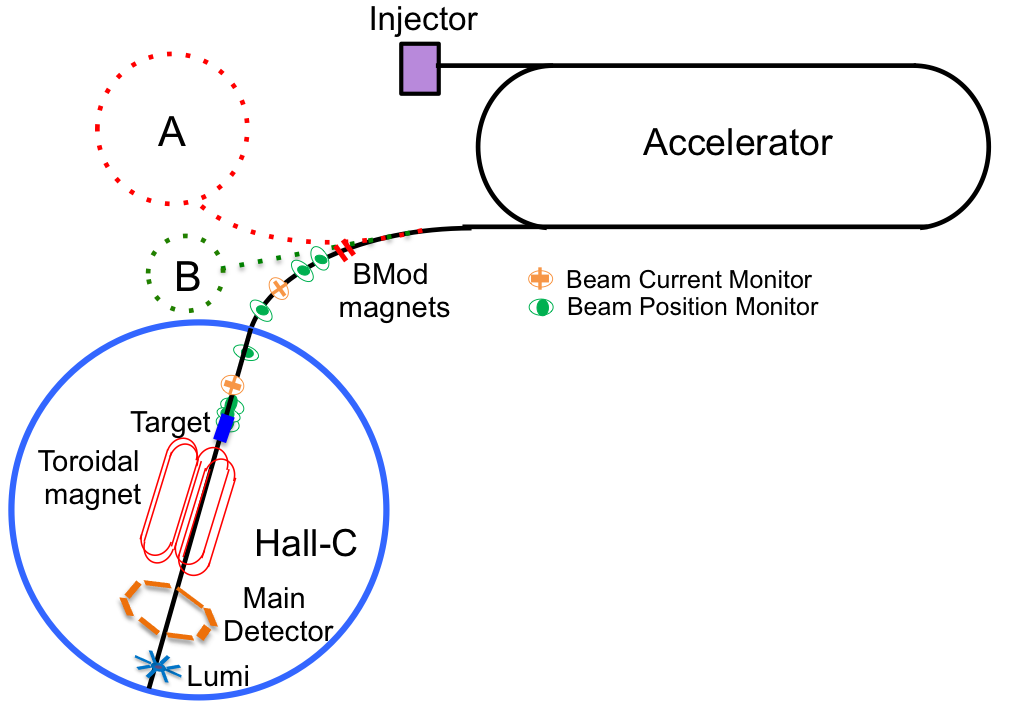
\includegraphics[width=15.0cm]{figures/BModAcceleratorSketch}
	\end{center}
	\caption
	[Simple schematic cartoon of the accelerator.]
	{Simple schematic cartoon of the accelerator. The beam modulation magnets are shown in Hall-C beamline. The BPMs, BCMs, and other key components of the experiment are shown in the Hall-C beamline. }
	\label{fig:BModAcceleratorSketch}
\end{figure}
\end{singlespace}


%%%%%%%%%%%%%%%%%%%%%%%%%%%%%%%%%%%%%%%%%%%%%%%%%%%%%%%%%%%%%
\section{Measurement Time vs Modulation Asymmetry}
\label{Measurement Time vs Modulation Asymmetry}
It is assumed that it would be helpful to measure the whole-detector sensitivities to 10\% accuracy every few days (provided it can be done using only a small fraction of the beam time and without beam strikes or halo scraping)~\cite{mack_communication}. 
%If the sensitivities prove to be stable, this would yield few percent errors by the end of the experiment. This is much better than one would need to regress out the helicity-correlated differences seen in the previous parity violating experiment HAPPEX~\cite{PhysRevLett.98.032301}.
Stable sensitivities would yield uncertainties of a few percent by the end of the experiment, which is much better than one would need to regress out the helicity-correlated differences seen in the previous parity violating experiment HAPPEX~\cite{PhysRevLett.98.032301}. However, frequent whole-detector sensitivity measurements might reveal important changes in the beam or the target cell position, the presence of an unmeasured beam parameter, or even a broken glue joint in the main detector. Furthermore, accurate single octant sensitivities (which would be obtained as a by-product) are an essential prerequisite to extract the $\sin\phi$ and $\cos\phi$ dependence which are characteristic of residual transverse beam polarization.

For the size and duration of the modulations discussed here, the natural beam jitter and the SEE BPM (section~\ref{Beam Position Monitor}) electronic noise of roughly 5~$\mu$m/$\sqrt{Hz}$ will be negligible. If this was not the case, measurement times would become much longer. This means that the uncertainty on the detector sensitivities is dominated by the statistical uncertainty on the detector false asymmetry. At nominal luminosity, the Q-weak experiment has a rate of 800~MHz/octant, hence the whole-detector statistical sensitivity, $dA$, is 12.5~ppm/$\sqrt{t}$(sec) or 1~ppm in 156.25~seconds. The clock times needed to measure a single beam sensitivity to 10\% are therefore given by

\begin{equation} \label{equ:time}
t (s) = \frac{1}{\textrm{DF}} \frac{\displaystyle\left(\frac{12.5~\textrm{ppm}}{A (\textrm{ppm})}\right)^2}{\left(\frac{\displaystyle dA}{\displaystyle A}\right)^{2}}  = \frac{1}{\textrm{DF}} \left(\frac{12.5~\textrm{ppm}}{A(\textrm{ppm})}\right)^2 \left(10\right)^{2} 
\end{equation}

%t (sec) = (1/DF)* (12.5 ppm/A(ppm))2/(dA/A)2 = (1/DF)*100*(12.5ppm/A(ppm))2 . 

\begin{singlespace}
\begin{table}[!h]
\begin{center}
  	\caption
	[Dead time calculation for beam modulation.]
  	{Dead time calculation for beam modulation. The clock time needed to measure detector sensitivity for a single parameter and how it varies with asymmetries are shown here.}
  \begin{tabular}{ c | c | c | c }
%    \hline
    \noalign{\hrule height 1pt}
    \multirow{2}{*}{Modulation asymmetry} & \multicolumn{3}{c}{Clock time required} \\
    \cline{2-4}
     & 10\% DF & 1\% DF & 0.1\% DF \\
     $\left[ \text{ppm}\right]$ & [Hours] & [Hours] & [Hours] \\ 
%    \hline
    \noalign{\hrule height 1pt}
    1 & 43 & 430 & 4300 \\ 
    10 & 0.43 & 4.3 & 43 \\ 
%    \hline
    \noalign{\hrule height 1pt}
  	\end{tabular}
  \label{tab:dead_time_modulation}
\end{center}
\end{table}
\end{singlespace}

Table~\ref{tab:dead_time_modulation} estimates required clock time for a 10\% measurement of a single beam sensitivity with different assumptions about the modulation asymmetry and the modulation duty factor. A modulation of 10~ppm would permit a measurement of all 5 sensitivities to 10\%, require about 1-10~calendar days, and have minimal negative impact on production duty cycle. For fixed uncertainty, smaller amplitudes would require at least quadratic increases in measurement time or duty factor (DF). For fixed measurement time and duty factor, smaller amplitudes would cause at least linear increases in the uncertainties. 

%%%%%%%%%%%%%%%%%%%%%%%%%%%%%%%%%%%%%%%%%%%%%%%%%%%%%%%%%%%%%
\section{Modulation Amplitude}
\label{Modulation Amplitude}
The next important step was to estimate the modulation amplitudes for beam position and angle necessary to achieve $A_\textrm{false}$ = 10~ppm. Detailed simulations on sensitivities have been performed using Geant-3 and is discussed in~\cite{jim_sensitivity}. The simulated single octant detector sensitivities are dominated by the interaction of e+p elastic scattering with the defining collimator, and are shown in the second column of Table~\ref{tab:beam_parameter1}.  Except for energy, the whole detector sensitivities were much smaller. They were much more complicated since they were determined by imperfect cancellation of the linear sensitivities due to broken symmetries (coil misalignment, radiator radial positions), plus quadratic sensitivities which depend on beam offsets. It is not unreasonable to disagree as to what expected suppression factor is to be used in going from single octant sensitivities to whole detector sensitivities. Therefore, the relatively conservative cancellation factor was assumed to be 50, which leads to the modulation amplitude for position, angle, and energy to generate 10~ppm whole detector asymmetry and are shown in Table~\ref{tab:beam_parameter1}.

\begin{singlespace}
\begin{table}[!h]
\begin{center}
  	\caption
	[A crude estimate of the modulation amplitudes to generate 10~ppm whole detector asymmetries.]
  	{A crude estimate of the modulation amplitudes to generate 10~ppm whole detector asymmetries.}
  \begin{tabular}{ l | c | c | c | c }
%    \hline
    \noalign{\hrule height 1pt}
    Beam      & Single & Assumed & Whole & Modulation\\
    Parameter & Octant & Cancellation    & Detector & Amplitude\\
      & Sensitivity &  & Sensitivity & for 10~ppm \\  
%   	\hline
    \noalign{\hrule height 1pt}
    Position  & 10~ppb/nm   & 50 & 0.2~ppb/nm   &	50~$\mu$m         \\ 
    Angle     & 30~ppb/nrad & 50 & 0.6~ppb/nrad & 20~$\mu$rad       \\
    Energy    & 1~ppb/ppb   & 1  & 1~ppb/ppb    & 10~ppm ($\sim$10~keV) \\ 
%    \hline
    \noalign{\hrule height 1pt}
  	\end{tabular}
  \label{tab:beam_parameter1}
\end{center}
\end{table}
\end{singlespace}

%Table~\ref{tab:beam_parameter1} crude estimates for the modulation amplitude needed to generate 10 ppm whole detector asymmetries. 
%A crude estimate of the modulation amplitude for position, angle, and energy to generate 10~ppm whole detector asymmetry are shown in  Table~\ref{tab:beam_parameter1}.
The estimated whole detector sensitivities were small. Compared to the Q-weak statistical uncertainty of $\sim$5~ppb, the beam parameter corrections resulting from the helicity-correlated differences seen in the previous parity violating experiments~\cite{PhysRevLett.98.032301} $\mathcal{O}$(1~nm, 0.1~nrad, 0.1~ppm in energy) were negligible. Alternatively, this means the allowable uncertainty in determining the beam sensitivity is 100\%, so a system capable of making a 10\% measurement on all 5 beam sensitivities every 1-10~days is apparently overkill. The real value of such a beam modulation system may be to detect undesired changes in the experiment, or as insurance in case the e+p sensitivities prove to be much larger than anticipated, or for those cases where the sensitivities are known to be much larger e.g., for elastic scattering on $^{9}$Be or $^{27}$Al window-like targets, inelastic scattering on LH$_{2}$ or $^{27}$Al, or the small angle scattering into the luminosity monitors. 


\begin{singlespace}
\begin{figure}[!h]
	\begin{center}
	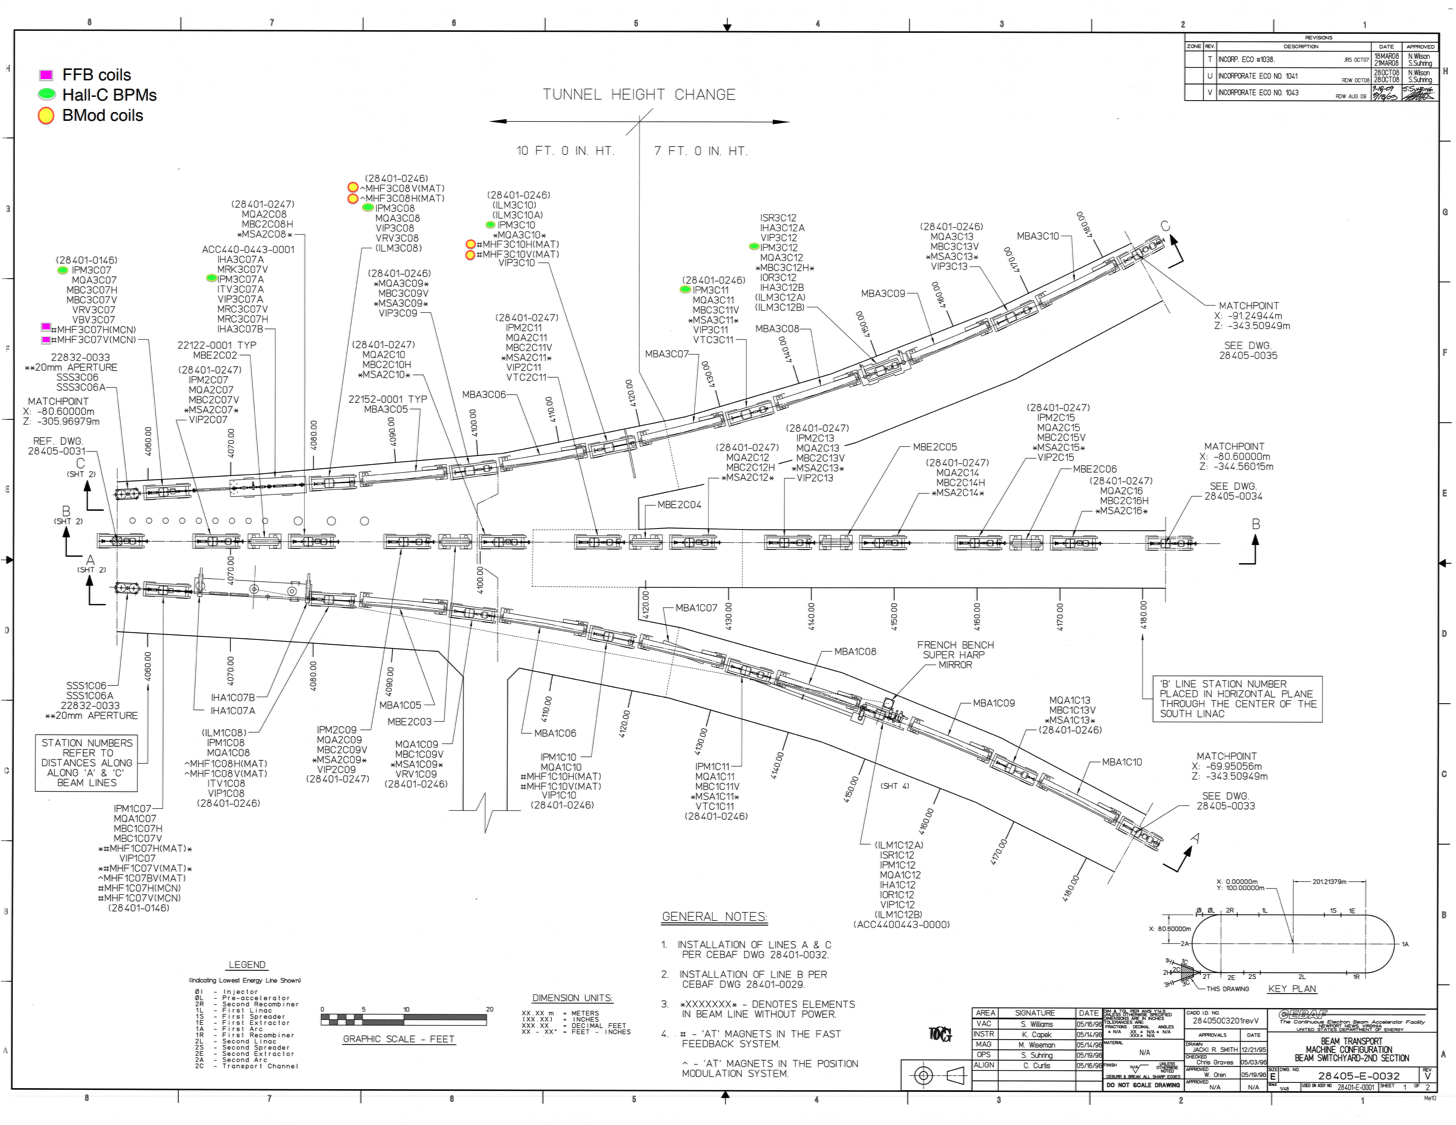
\includegraphics[width=15.0cm]{figures/beamline_songsheet}
	\end{center}
	\caption
	[Jefferson Lab and its beamline schematic for all three experimental halls.]
	{Jefferson Lab and its beamline schematic for all three experimental halls using Computer Aided Design (\newnot{symbol:CAD}CAD\index{CAD}) drawings (informally referred as songsheets at Jefferson Lab) are shown. Beam modulation magnets, fast feed back coils, and BPMs in the Hall-C beamline are labeled separately.}
	\label{fig:beamline_songsheet}
\end{figure}
\end{singlespace}

%%%%%%%%%%%%%%%%%%%%%%%%%%%%%%%%%%%%%%%%%%%%%%%%%%%%%%%%%%%%%
\section{Optics Calculation}
\label{Optics Calculation}
A software written by Valery Lebedev for linear and non-linear optics calculations, OptiM~\cite{OPTIM}, and an input deck prepared by Jay Benesch~\cite{jay_communication} (JLab) were used to simulate the Hall-C beamline (3C). The 3C beamline was substantially modified before Q-weak to accommodate the Compton polarimeter. A schematic view of the Hall-C beamline (songsheet\footnote{The CAD drawings were informally referred as songsheets at Jefferson Lab. The CAD annotation is static. Only element names are shown in the drawings.}) along with the other halls are shown in Figure~\ref{fig:beamline_songsheet}.
%, so the (undocumented) parity infrastructure left over from the G0 experiment would have been toast even if we had planned to retain it.  
%We utilize the OPTIM program written by Valery Lebedev~\cite{OPTIM} and an input deck prepared by Jay Benesch~\cite{jay_communication} for Hall-C beamline.  The 3C beamline will be substantially modified before $Q_{weak}^{p}$ to accomodate a Compton polarimeter, so the (undocumented) parity infrastructure left over from the G0 experiment would have been toast even if we had planned to retain it.  
The goal for the beam modulation system was to achieve robust modulation in $X$, $X^{'}$, $Y$, $Y^{'}$, and $E$ at the target. These modulations do not have to be strictly pure, but they have to be linearly independent so that have solutions for the individual sensitivities. The asymmetries from position modulations were an order of magnitude larger than the corresponding asymmetries from angle modulations for similar sized magnet kicks in the Q-weak and will be discussed in later sections of this chapter.
This fact, plus the relatively large statistical noise in the detector asymmetries, plus the certainty of small drifts in the optics, suggested that mixed mode modulation is unlikely to be robust. Running times and uncertainties were also quite difficult to estimate for the mixed mode modulation. Therefore, relatively pure modulations in which $\sim$90\% of the asymmetry arises from the variable of interest was attempted to produce.
%Strictly speaking, these modulations do not have to be pure, but they have to be linearly independent so that one can solve for the individual sensitivities. However, we'll see below that for similar sized magnet kicks in Qweak, asymmetries from position modulations are an order of magnitude larger than the corresponding asymmetries from angle modulations. This fact, plus the relatively large statistical noise in the detector asymmetries, plus the certainty of small drifts in the optics, suggest to us that "mixed mode" modulation is unlikely to be robust. Running times and uncertainties would also be quite difficult to estimate in the case of mixed mode modulation. Therefore, we will attempt to produce relatively pure modulations in which 90\% of the asymmetry arises from the variable of interest.
%  
%There were significant constraints on where perturbing coils can be located. One absolute requirement was that coils be located upstream of the high dispersion point at 3C12 (the center of the 3C arc) so that modulations in X, X$^{'}$, and E can be disentangled. Another highly desirable constraint was that the coils be located downstream of any expected deviations from design optics. Accelerator operations agreed to complete matching in 3C beamline by MQA3C08, the beginning of the 3C arc dipole string. Considerations of robustness and purity therefore excluded regions upstream of this, leaving only only the first half of the 3C arc as a potential site for coils. 


\subsection{Simulation using OptiM}
\label{Simulation using OptiM}
The main OptiM deck~\cite{optim_deck} contain the information about the location, field strength, size, orientation etc. for each component of the Hall-C beamline.
%The main OptiM deck~\cite{optim_deck} contain all the detailed information about all the elements in the Hall-C beamline. It has the information like location of the beamline, field strength, size, orientation etc. 
%One can also get the transfer matrices between any two beamlime elements using the software. It also produces simulated trajectories through the beamline from one element to another. 
%The OptiM deck was used to produce simulated trajectories form beam modulation magnet pair at the beginning of Hall-C beamline to the Q-weak target
%The simulated trajectories form beam modulation magnet pair at the beginning of Hall-C beamline to the Q-weak target was produced .
%We used OptiM to give us simulated trajectories form beam modulation magnet pair at the beginning of Hall-C beamline to the Q-weak target. We also changed our basis of calculation from beam modulation coil co-ordinate to Q-weak target co-ordinate using OptiM.
The OptiM deck was used to obtain transfer matrices, obit excursion, beta functions, and simulated trajectories between any two beamlime elements in forward or inverse direction.

\begin{singlespace}
\begin{figure}[!h]
	\begin{center}
	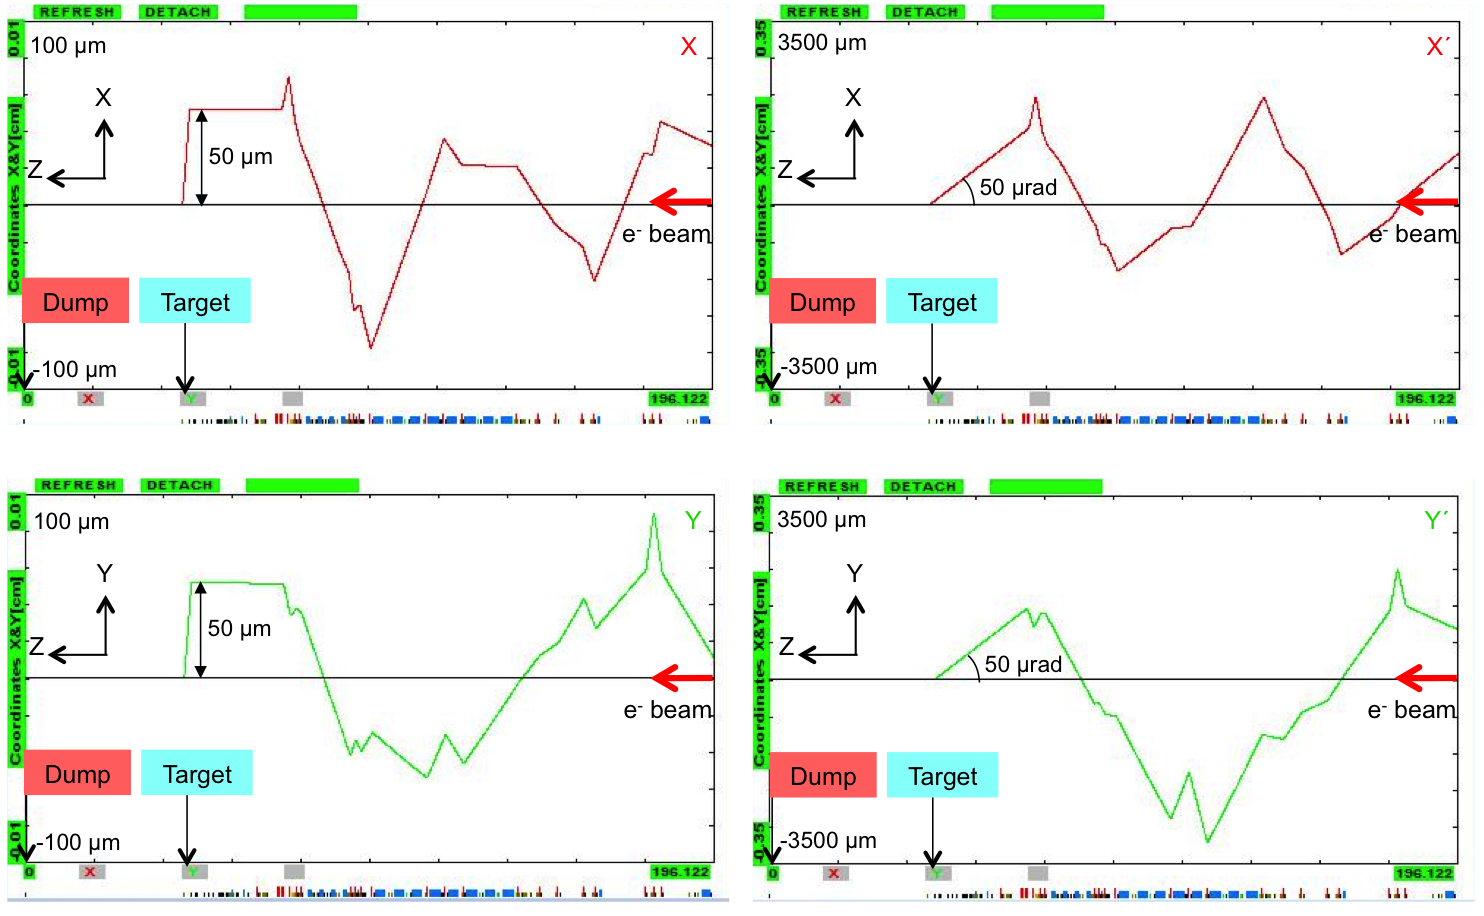
\includegraphics[width=15.0cm]{figures/BModInverseBeamline}
	\end{center}
	\caption
	[Inverse orbit excursions simulation from OptiM.]
	{Inverse orbit excursions simulation from OptiM. The direction of the beam is from right to left. The ting blue and red boxes on the horizontal axis at the bottom of the figures are dipoles and quadrupoles, respectively. The location of the target and beam dump are also marked. The orbit excursion for the relatively pure $X$, $X^{\prime}$, $Y^{\prime}$ and $Y$ motion at the target are shown in the four panels (from top left in clock wise direction).}
	\label{fig:BModInverseBeamline}
\end{figure}
\end{singlespace}

\subsection{Inverse Beamline}
\label{Inverse Beamline}
An insightful starting exercise was to start with a pure position or angle deviation at the target and use OptiM to send tracks in the upstream direction which was named as inverse beamline or orbit. Figure~\ref{fig:BModInverseBeamline} shows the orbit from the target to the Lambertson (beginning of the 3C line). All 4 panels have the same qualitative features: the beam moves to the right with piece-wise continuous motion, there is a discontinuity at each quadrupole location, and there is at least one zero crossing. The reason this inverse trajectory is so interesting is that, due to time-reversal invariance of electromagnetic interactions, it provides the information about how to perturb a forward beam to obtain a pure position or angle change at the target. As long as the inverse orbit stays inside the beampipe, such a figure is an existence proof that pure modulation at the target is possible with a forward beam. 


\begin{singlespace}
\begin{figure}[!h]
	\begin{center}
	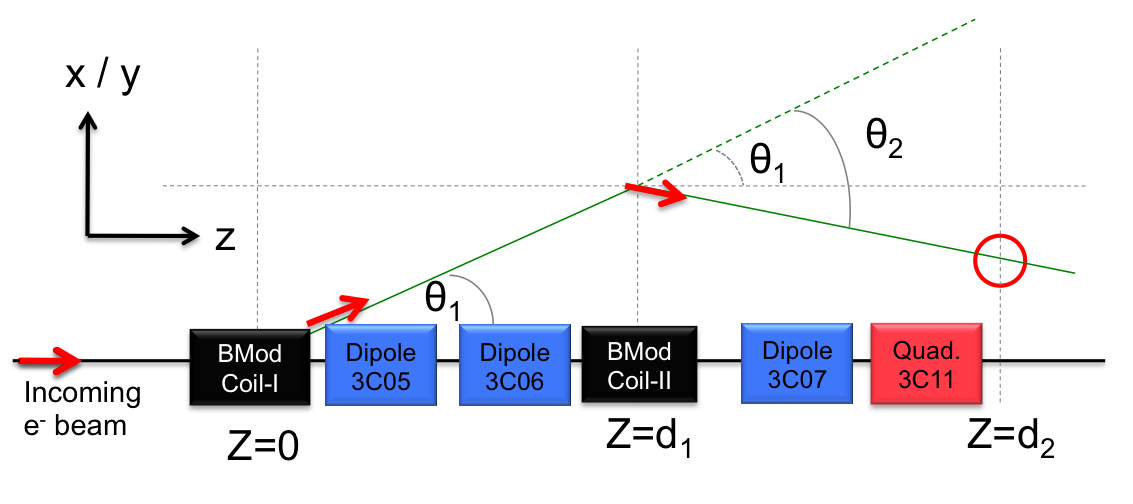
\includegraphics[width=15.0cm]{figures/BModDrawing}
	\end{center}
	\caption
	[A sketch of beam modulation concept.]
	{A sketch of beam modulation concept. A pair of magnets (Z=0 and Z=d$_{1}$) with opposite kick were used to match a trajectory at any arbitrary point (Z=d$_{2}$) in the beamline. There were two big dipoles between the modulation magnets. Using simple algebra $\theta_{1}$ and $\theta_{2}$ can be expressed in terms of position and angle at the match point. Hence required filed integral in the beam modulation magnets can be calculated to generate a particular trajectory (details of the calculation in APPENDIX~\ref{BEAM MODULATION 2}).}
	\label{fig:BModDrawing}
\end{figure}
\end{singlespace}

\subsection{Forward Beamline with Position or Angle Kicks}
\label{Forward Beamline with Position or Angle Kicks}
The simplest way to perturb an arbitrary forward beam onto the magic trajectory obtained using inverse beamline is to kick the beam with a single small dipole at one of the zero crossings.  However, if driving coils were restricted to the first half of the 3C arc, this strategy was not feasible because there was only one zero crossing in that region (corresponding to pure $X^\prime$ modulation), with no zeros corresponding to $X$, $Y$, or $Y^\prime$ modulation.  A better approach was then suggested by Mike Tiefenback~\cite{tiefenback_communication}, similar to that used in the JLab Fast Feedback System (\newnot{symbol:FFB}FFB\index{FFB})~\cite{jlab_ffb1,jlab_ffb2}. As schematically shown in Figure~\ref{fig:BModDrawing}, pairs of separated coils could be used to take an arbitrary forward ray, offset its position and angle, and re-inject it along the appropriate trajectory to produce a pure position or angle change at the target. Detailed OptiM solutions for forward rays are shown in Figure~\ref{fig:BModForwardBeamline} for a pair of coils separated by 9.5~m. Note that position modulation of $\pm$~250~$\mu$m at the target yields orbit deviations of similar magnitude in the beamline, while angle modulation of $\pm$~50~$\mu$rad at the target yields orbit deviations of up to 3~mm.  The size of the latter orbit deviations is large enough to cause some concern about scraping of the beam or halo. (The impact on the Compton polarimeter laser $X$ electron beam lock has not been examined.) 
Hence the angle kick was reduced by an order of magnitude smaller to match the size of the orbit deviations. This might be a better match to the size of natural beam jitter, but the time required in Table~\ref{tab:beam_parameter1} for a single 10\% measurement would increase by at least a factor of 100. The field integrals for that yielded pure modulations at the Q-weak target were calculated using most updated available OptiM deck~\cite{optim_deck} and are shown in Table~\ref{tab:beam_parameter}.
These field integrals were converted to currents using the measured MAT coil field constant of 330~G-cm/A. This two-coil scheme was very convenient, as any changes in the 3C line was easily simulated for the modulation system by re-tuning the ratio of coil currents without having to move coils.
%It is conceivable that the 3C beamline design optics will be revised yet again in order to optimize operation of the new Compton polarimeter.  Fortunately, in this two-coil scheme, we would be able to simply retune the ratio of coil currents without having to move coils. 

\begin{singlespace}
\begin{figure}[!h]
	\begin{center}
	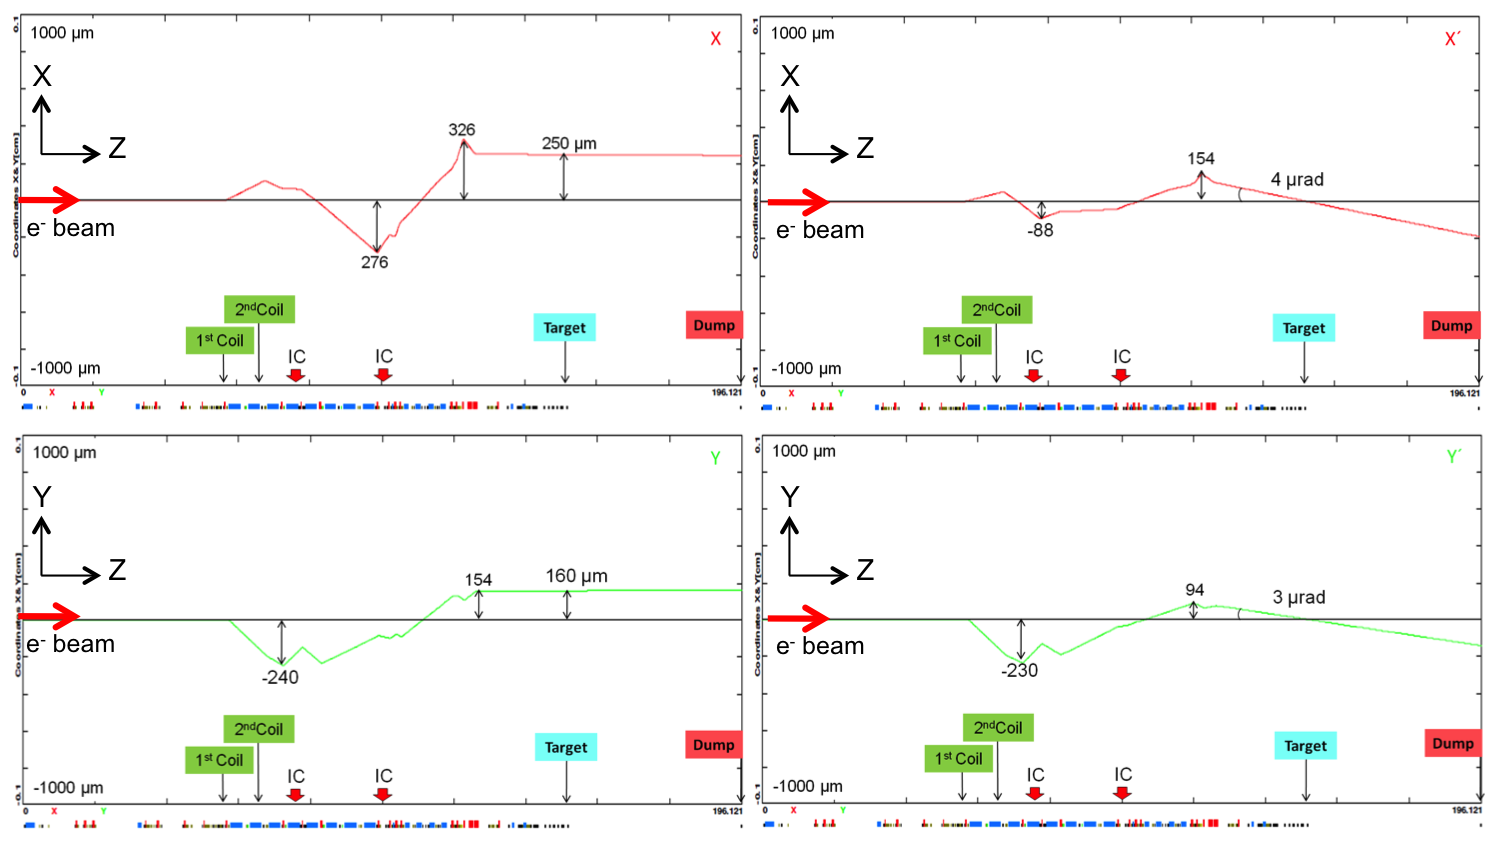
\includegraphics[width=15.0cm]{figures/BModForwardBeamline}
	\end{center}
	\caption
	[Forward orbit excursions simulation from OptiM.]	
	{Forward orbit excursions simulation from OptiM. Beam moves from left to right. The ting blue and red boxes on the horizontal axis at the bottom of the figures are dipoles and quadrupoles, respectively. Simulated location of the modulation magnets and recommended location for ion chambers are shown in the figures. The forward orbit excursion for the relatively pure $X$, $X^{\prime}$, $Y^{\prime}$ and $Y$ motion at the target are shown in the four panels (from top left in clock wise direction).}
	\label{fig:BModForwardBeamline}
\end{figure}
\end{singlespace}



\begin{singlespace}
\begin{table}[!h]
\begin{center}
  	\caption
	[Required field integrals for the modulation dipole pair from OptiM.]
  	{Required field integrals for the modulation dipole pair to generate relatively pure position and angle at the target from OptiM are shown here. Coil currents to produce such field integrals are calculated. The ratio between coil current in 2nd and 1st coil is defined as tune parameters. The negative tune parameters signifies the out of phase current in the two coils. }
  \begin{tabular}{ c | c | c | c | c | c | c }
%    \hline
    \noalign{\hrule height 1pt}
    Beam      & Amplitude & $I_1$    & $\int\vec{B}\bullet\vec{dl_{1}}$ & $I_2$ & $\int\vec{B}\bullet\vec{dl_{2}}$ & Tune  \\
    Parameter & for 10~ppm & [A] & [G-cm] & [A] & [G-cm] & \\ 
%    \hline
    \noalign{\hrule height 1pt}
%		X	& 50~$\mu$m	& 0.026	& 8.5	& -0.026 & -8.5 & -1.00\\ \hline
%		X$^\prime$	& 50~$\mu$rad	& 0.026	& 8.5	& -0.026 & -8.5 & -1.00\\ \hline
%		Y	& 50~$\mu$m	& 0.026	& 8.5	& -0.026 & -8.5 & -1.00\\ \hline
%		Y$^\prime$	& 50~$\mu$rad	& 0.026	& 8.5	& -0.026 & -8.5 & -1.00\\ \hline
		$X$	& 250~$\mu$m				& 0.159	& 52.4		& -0.372 	& -122.9 & -1.875\\
		$X^\prime$	& 4~$\mu$rad	& 0.554	& 183.0	& -1.872 	& -618.0 & -3.864\\ 
		$Y$	& 160~$\mu$m				& -0.242	& -80.0	& 0.060 	& 20.0 & -0.367\\ 
		$Y^\prime$	& 3~$\mu$rad	& -1.606	& -530.0	& 0.771 	& 254.0 & -0.489\\ 
%		\hline
    \noalign{\hrule height 1pt}
  	\end{tabular}
  \label{tab:beam_parameter}
\end{center}
\end{table}
\end{singlespace}

\subsection{Forward Rays with Energy Kick}
\label{Forward Rays with Energy Kick}
The beam energy was modulated using a superconducting RF cavity in the South Linac of the accelerator. The effect of a simulated 10~ppm energy kick from OptiM is shown in Figure~\ref{fig:BModEnergy}.  At 3C12, the point of highest dispersion (the middle of the 3C arc), the induced motion is shown by a 41~$\mu$m red spike.  From a comparison of Figures~\ref{fig:BModForwardBeamline} and \ref{fig:BModEnergy}, it is pretty clear that energy changes could not possibly be confused with position or angle changes. Further downstream in the beamline, the small green bump represents the dispersion inside the vertically bending Compton chicane. Because of the lower dispersion, the induced motion in the Compton was only about 5~$\mu$m, much smaller than the nominal JLab electron beam rms width. 
The energy change at the target was identified in terms of change in beam position at 3C12 and at any arbitrary location. A pair of BPMs at the beginning or the end of the 3C arc would seem to be the most natural choice for energy change measurement. Any two $X$ BPMs on the beamline could be used as long as the magnifications were favorable. But there were advantages to work in terms of target position ($X_{T}$) and angle ($X^{\prime}_{T}$) because: 1) these were the coordinates that were used in the simulations to estimate the beam sensitivities, and 2) there were seven BPMs in the drift region upstream of the target which provided flexibility to determine $X_{T}$ and $X^{\prime}_{T}$ with relatively high accuracy~\cite{nur_linear_reg}. Previous experiments typically used two BPMs in front of the target, thus lacking the above two advantages.
The position or angle at 3C12 in terms of target parameters can be expressed as

\begin{equation} \label{equ:energy1}
\overleftrightarrow{X}_\textrm{3C12} = \underline{M} \overleftrightarrow{X}_{T}
\end{equation}

Expanding the Eq.~\ref{equ:energy1}

\begin{equation} \label{equ:bmodMatrix1}
    \begin{bmatrix}
       X\\[0.3em]
       X^{\prime}\\[0.3em]
       Y\\[0.3em]
       Y^{\prime}\\[0.3em]
       \frac{dE}{E}\\[0.3em]
    \end{bmatrix}_\textrm{3C12}
	=
	\begin{bmatrix}
       M_{11} & M_{12} & M_{13} & M_{14} & M_{15} \\[0.3em]
       M_{21} & M_{22} & M_{23} & M_{24} & M_{25} \\[0.3em]
       M_{31} & M_{32} & M_{33} & M_{34} & M_{35} \\[0.3em]
       M_{41} & M_{42} & M_{43} & M_{44} & M_{45} \\[0.3em]
       M_{51} & M_{52} & M_{53} & M_{54} & M_{55} \\[0.3em]
    \end{bmatrix}
    \begin{bmatrix}
       X\\[0.3em]
       X^{\prime}\\[0.3em]
       Y\\[0.3em]
       Y^{\prime}\\[0.3em]
       \frac{dE}{E}\\[0.3em]
    \end{bmatrix}_{T}
\end{equation}

where the matrix elements were obtained from~\cite{optim_deck} and can be written as

%\begin{equation} \label{equ:bmodMatrix2}
%M	=
%	\begin{bmatrix}
%       0.69 & -928 & -3\times 10^{-16} & 2\times 10^{-12} & 411 \\[0.3em]
%       -5\times 10^{-4} & 2.1 & 6\times 10^{-19} & 3\times 10^{-15} & -0.5 \\[0.3em]
%       -1\times 10^{-16} & 3\times 10^{-14} & -0.60 & -3.5\times 10^{4} & -1 \\[0.3em]
%       -5\times 10^{-19} & -2\times 10^{-16} & -6\times 10^{-4} & -5 & -1\times 10^{-3} \\[0.3em]
%       0 & 0 & 0 & 0 & 1 \\[0.3em]
%    \end{bmatrix}
%\end{equation}

\begin{equation} \label{equ:bmodMatrix2_1}
M	=
	\begin{bmatrix}
       0.69 & -928 & 0 & 0 & 411 \\[0.3em]
       -5\times 10^{-4} & 2.1 & 0 & 0 & -0.5 \\[0.3em]
       0 & 0 & -0.60 & -3.5\times 10^{4} & -1 \\[0.3em]
       0 & 0 & -6\times 10^{-4} & -5 & -1\times 10^{-3} \\[0.3em]
       0 & 0 & 0 & 0 & 1 \\[0.3em]
    \end{bmatrix}
\end{equation}

Using Eq.~\ref{equ:bmodMatrix1} and~\ref{equ:bmodMatrix2_1}, the energy change at the target can be written in terms of horizontal position change at 3C12, and horizontal position and angle changes at the target as 

\begin{equation} \label{equ:energy2}
\Delta\left(\frac{dE}{E} \right)_{T} = \frac{1}{M_{15}}\Delta X_\textrm{3C12} - \frac{M_{11}}{M_{15}}\Delta X_{T} - \frac{M_{12}}{M_{15}}\Delta X^{\prime}_{T}
\end{equation}

More detailed calculation about the energy modulation can be found in~\cite{nur_bm_energy}.

\begin{singlespace}
\begin{figure}[!h]
	\begin{center}
	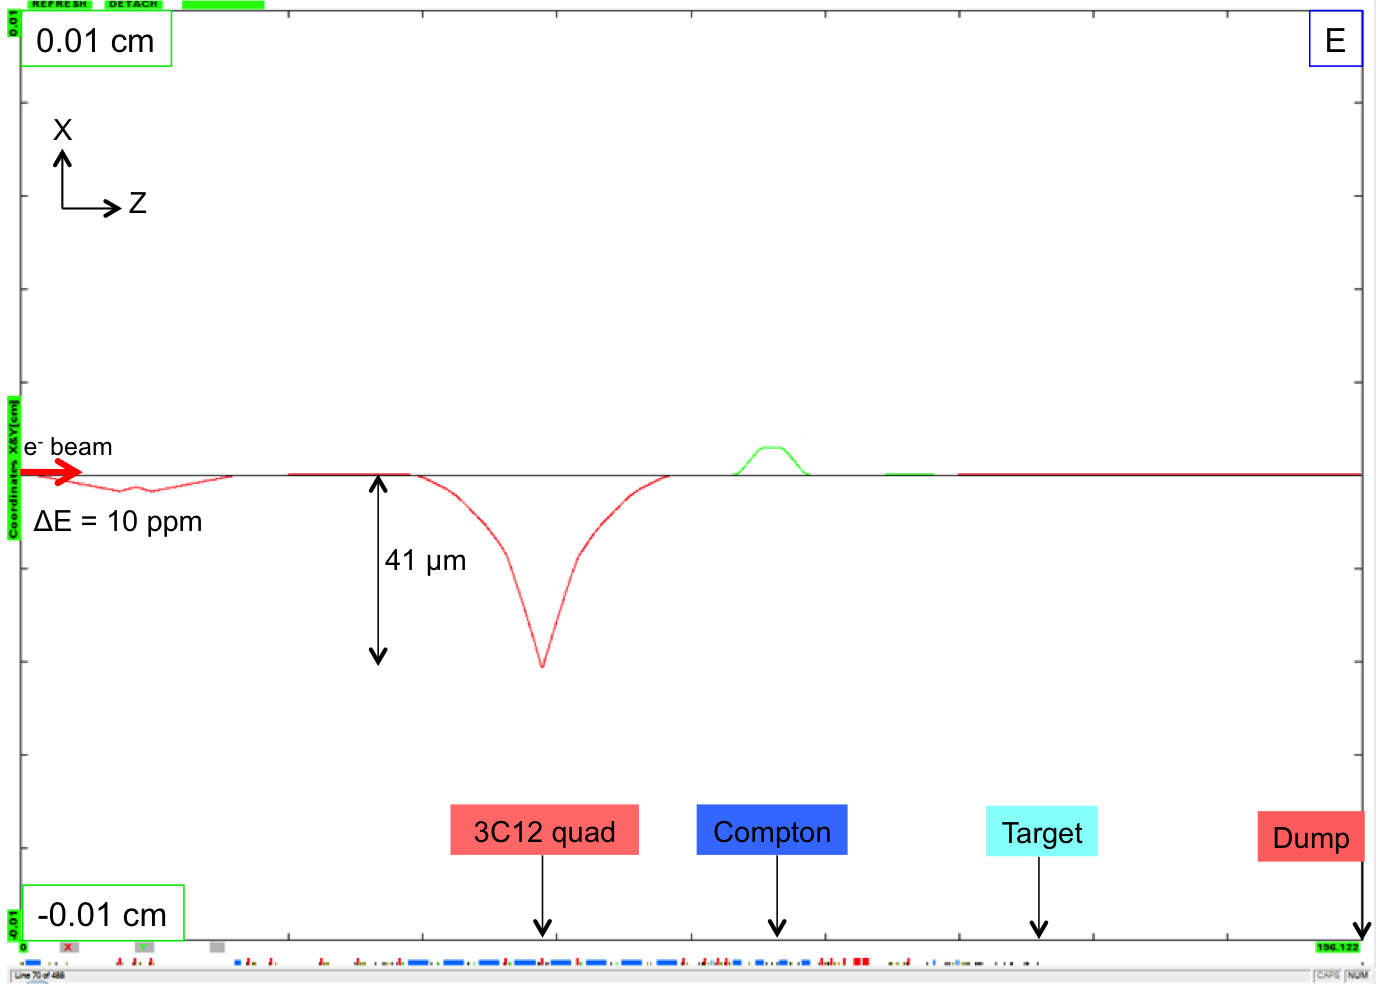
\includegraphics[width=10.0cm]{figures/BModEnergy}
	\end{center}
	\caption
	[Forward orbit excursions simulation for energy modulation from OptiM.]
	{Forward orbit excursions simulation for energy modulation from OptiM. Beam moves from left to right. The energy was changed by 10~ppm using a horizontal corrector in the simulation. The pronounced horizontal position (red) change of 41~$\mu$m at the middle of the arc is due to the energy change of 10~ppm. A small vertical position (green) bump can be identified at the Compton region.}
	\label{fig:BModEnergy}
\end{figure}
\end{singlespace}


\begin{singlespace}
\begin{figure}[!h]
	\begin{center}
	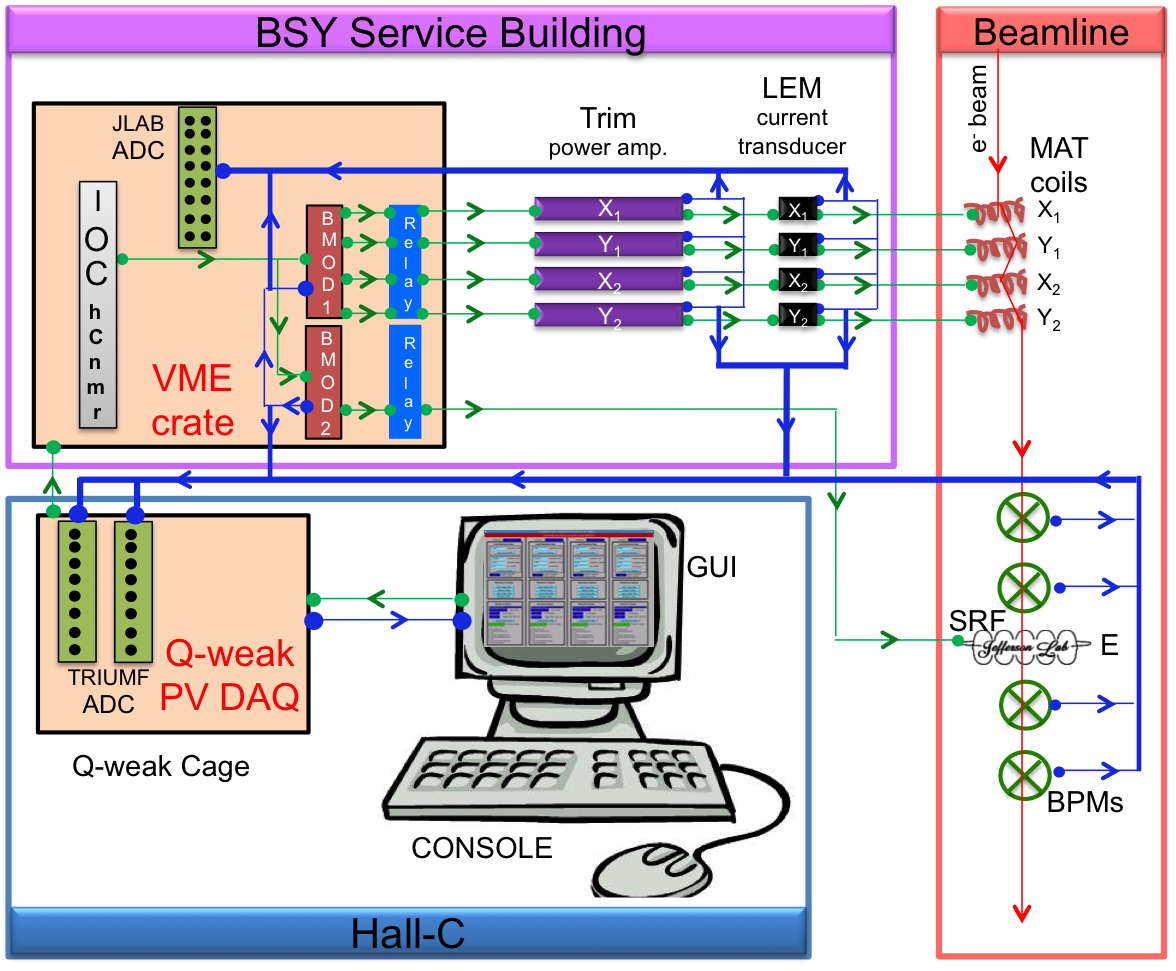
\includegraphics[width=15.0cm]{figures/BModHardwareSketch}
	\end{center}
	\caption
	[Beam modulation hardware sketch.]
	{Beam modulation hardware sketch. BMod hardware spans three different regions: BSY service building, accelerator beamline, and Hall-C. In BSY service building there were two VME-4145 signal generators controlled by an IOC (iochcnmr). The sinusoidal signals from signal generator were sent to Trim-I power amplifier, and amplified signals were sent to two pairs of MAT coils and one SRF cavity (SL20 vernier) in the beamline. The read-backs from signal generators, power amplifiers, current transducers, BPMs, and cavity were sent to two TRIUMF-made ADCs at Q-weak cage and one JLab-made ADC at BSY service building. The drive or input signals are shown by green and read-backs by blue lines respectively. In order to trigger the process, a signal from parity violating DAQ in the Hall-C counting house were sent to the IOC.}
	\label{fig:BModHardwareSketch}
\end{figure}
\end{singlespace}

%%%%%%%%%%%%%%%%%%%%%%%%%%%%%%%%%%%%%%%%%%%%%%%%%%%%%%%%%%%%%
\section{Beam Modulation Hardware}
\label{Beam Modulation Hardware}

The hardware of the beam modulation system spans three different regions: BSY service building, accelerator beamline, and Hall-C. In the BSY service building, there were two signal generators controlled by an IOC. The sinusoidal signals from signal generator were sent to power amplifier, and the amplified signals were sent to two pairs of air core coils and one SRF cavity in the beamline. The read-backs from signal generators, power amplifiers, current transducers to measure the coil current, and BPM responses were sent to two sets of ADCs at the Q-weak cage at Hall-C counting house and at BSY service building to monitor the system and to perform further analysis. A trigger from parity violating DAQ in the Hall-C counting house were sent to the IOC at BSY service building to start the process. The schematic diagram of the beam modulation hardware is shown in Figure~\ref{fig:BModHardwareSketch}.

\subsection{Air-Core Coils}
\label{Air-Core Coils}
Two pairs of JLab MAT(HF) air-core coils were used to perturb the electron beam for the modulation system as they produced sufficient field integral, were readily available, and were compact enough (10~cm) to be inserted easily in almost anywhere in the beamline. Their properties have been measured and summarized by Sarin Philips in~\cite{DocDB:sarin_979}. The MAT coils were calibrated in bench test and the most critical parameters are summarized in Table~\ref{tab:modulation_magnet}. The total impedance of the coil was related to the frequency ($f$) as $X_\textrm{total}$ = 1.6~$\Omega$ + 2$\pi f$(0.0038~H). The reduction in field due to the skin effect in a standard stainless steel beampipe was determined to be roughly 10\% at 1~KHz, and less than a few percent at nominal frequency of 125~Hz. The skin effect was ignored as the used frequency of the sinusoidal modulation was 125~Hz, which was constrained by the power amplifier (see section~\ref{Trim Power Amplifier}). 

%We plan to use JLab MAT(HF) air-core coils because they have sufficient field integral, they are readily available due to a recent switch of the FFB system to lower inductance coils, and they are short so can be easily tucked in almost anywhere.  Their properties have been measured and summarized in an Excel file by Sarin Philips (JLab). [ref: http://qweak.jlab.org/doc-public/ShowDocument?docid=979 ] The most critical parameters are summarized in Table 4. (For reference, the total impedance is $X_{tot}$ = 1.6 $\Omega$ + 2$\pi$f(0.0038H).)  S. Philips also determined the reduction in field due to the skin effect in a standard stainless steel beampipe to be roughly 10\% at 1 KHz, and less than a few percent at our nominal frequency of 250 Hz. The amplifiers we plan to use limit us to sinusoidal modulation at 250 Hz, so we will ignore the skin effect henceforth.

%\begin{singlespace}
%\begin{table}
%\begin{center}
%  \begin{tabular}{| c | c | c | c | c | c |}
%    \hline
%    Magnet Parameter & Magnet Constant (B/I) & $\int\vec{B}\bullet\vec{dl}$ = (B/I) x Length & Length & Inductance & Resistance \\ \hline
%     Value & 33 G/Amp & (330 G-cm/Amp) * I & 10 cm & 3.8 mH & 	1.6 $\Omega$ \\ \hline
%  	\end{tabular}
%  	\caption[Beam modulation magnet details]{Beam modulation magnet details}
%  \label{modulation_magnet1}
%\end{center}
%\end{table}
%\end{singlespace}

\begin{singlespace}
\begin{table}[!h]
\begin{center}
  	\caption
  	[Basic properties of the air core MAT coils used for the beam modulation system.]
  	{Basic properties of the air core MAT coils used for the beam modulation system.}
  \begin{tabular}{ l | c }
%    \hline
    \noalign{\hrule height 1pt}
    Magnet Parameter & Value \\ 
%    \hline
    \noalign{\hrule height 1pt}
		Magnet Constant ($B$/$I$) &	33 G/A \\ 
	 	$\int\vec{B}\bullet\vec{dl}$ = (B/I) $\times$ Length &	(330 G-cm/A)$\times$I \\ 
		Length &	10 cm \\ 
		Inductance &	3.8 mH \\ 
		Resistance &	1.6 $\Omega$ \\ 
%		\hline
    \noalign{\hrule height 1pt}
  	\end{tabular}
  \label{tab:modulation_magnet}
\end{center}
\end{table}
\end{singlespace}

\subsection{IOC}
\label{IOC}
A VME based Input Output Controller (IOC) \textit{hcnmr} at BSY service building was used to operate the beam modulation system.
IOC was a chassis containing a processor, various input/output (I/O) modules, and VME modules that provide access to other I/O buses~\cite{epics_ioc}. The IOC used to establish communication with two VME 4145 Signal Generator boards through two patch panels and controlled the drive signal of VME 4145 board via a database access library that works on Unix, vxWorks\footnote{VxWorks is a real-time operating system developed as proprietary software by Wind River Systems of Alameda, California, USA. First released in 1987, VxWorks is designed for use in embedded systems.}, and EPICS databases. 

\subsection{VME 4145 Signal Generator}
\label{VME 4145 Signal Generator}
Two GE Fanuc Intelligent Platforms' VME-4145 programmable function generator boards~\cite{manual_vmivme4145} were used to drive two pairs of MAT coils (shown in Figure~\ref{fig:BModHardwareSketch}). The VME-4145 has an analog output board that provides four high-quality analog output channels with 16-bit resolution. Each output has a dedicated Digital-to-Analog Converter (DAC), and can source or sink 10~mA $\pm$ 10~V. Each channel has a dedicated 64 Kword\footnote{KWord is a deprecated word processor and a desktop publishing application, part of the KOffice suite~\cite{website:kword}.} waveform buffer. Each buffer may be segmented to provide independent subwaveforms. The unit was capable of downloading an arbitrary bipolar waveform and then replay it. Any arbitrary waveform like square, sine, triangle, and sawtooth may be programmed. Two pairs of MAT coils were driven using sine waveform from the four channels of the first VME-4145 board. Only two channels of the second board were used. One channel was used to drive superconducting RF cavity for energy modulation with a sine waveform and the other channel was used to produce a ramp (sawtooth) wave to monitor the phase of the all five drive signals. Each waveform was generated start to finish and then the next was seamlessly started. All of the waveforms were preloaded before waveform generation begins. An external trigger input from Q-weak main DAQ was used to start playback of the waveform. This feature allowed to trigger the drive signal and ramp wave channels to synchronize in phase. The boards were programmed to run in the continuous mode (Type II) which scanned the waveform table, ran for 510~cycles and then halted. The next cycle started again when the boards were triggered from the Q-weak DAQ. 


\subsection{Relay Board}
\label{Relay Board}
Two sets of JLab-made 16-channel relay output register modules~\cite{jlab_relay} were used to make it easy to keep everything safe and tidy for the modulation system. The board consists of four 16-bit registers used to control 16 relays and read-back status information. The front panel contains indicator LED's for power, heartbeat and relay on/off status. Relay contacts are brought out on a 50-pin D connector.
A DC shift of $\sim$0.015~V was observed in the sinusoidal drive signal due to the relay boards which seem to have no effect on the driven coils (more details in~\cite{presentation:nur_bmod_1312}).

\subsection{Trim Power Amplifier}
\label{Trim Power Amplifier}
Four 1 to 12~A series pass regulator power supplies, known as Trim Card I, were used as power amplifiers to control two pairs of the MAT dipoles for the beam modulation system. The Trim-I was programmable, 200~W, bipolar, power supply and was realized as a single plugin circuit board, approximately with dimensions 9$\inchsign\times$20$\inchsign$. A new generation plug-compatible supply Trim-II was being developed to replace the Trim-I by JLab accelerator group~\cite{1591576}. Thirty two Trim cards were housed in card-cages within a single rack (BS04B14) at BSY service building. But only four of those cards were used for the modulation system and the rest were used to power other components in the beamline. The Trim cards consisted of a Motherboard which helped to interconnect all the daughter cards, distribute power to the daughter cards, and house the power amplifier section (shown in Figure~\ref{fig:BModTestHardware}). A 48-pin connector, mounted on the rear apron, was used to engage a mating connector in the card cage where $\pm$~27~V bulk power, 5~V power, and RS-485 communication were derived. External programming commands and data read-backs were exchanged with the EPICS via a RS-485 data link. The cards had a display module in the front connected to a digital temperature sensor which was used to set warning flags or shutdown the trim card in case of overheating. The Trim cards setup suffers from a discontinuity when conduction changes from the positive to negative pass bank transistor arm as the output passes though the zero point. This effect was suppressed by the feedback loops, and was problematic for fast ramps or step changes. The drive signal for the modulation was constrained by this phenomena, and instead of square or triangular waves, sinusoidal wave was chosen. Originally, the Trim cards were designed to operate in the DC regime, but managed to amplify up to 250~Hz smooth sine wave linearly. Near the higher frequency and saturation current, the Trim cards locked itself to prevent any potential damage. 

%Jefferson Lab uses 1 to 12 A series pass regulator power supplies, known as Trim Card I, to control approximately 1900 X-Y dipole steering magnets, focusing quadrapole magnets, and solenoids throughout CEBAF. This programmable, 200 W, bipolar, power supply has performed reliably for over 12 years. However, the rapid evolution of electronic components has resulted in its obsolescence and the need for piggyback adapter boards to replace discontinued technologies. New additions to the CEBAF beam line have been common throughout its evolution. These devices often require different output voltages, output currents, and programming characteristics such as specific current-ramp profiles. The Trim Card I is limited in its capability to incorporate the needs of these new devices. The card is also lacking diagnostic and self-check features that would facilitate quick diagnosis and shorter repair times. A new generation plug-compatible supply is being developed to replace the Trim Card I. The redesigned Trim Card II addresses the issues of obsolescence, flexibility, and diagnostics by taking a modular design approach and using up-to-date components [2, 3].

\begin{singlespace}
\begin{figure}[!h]
	\begin{center}
	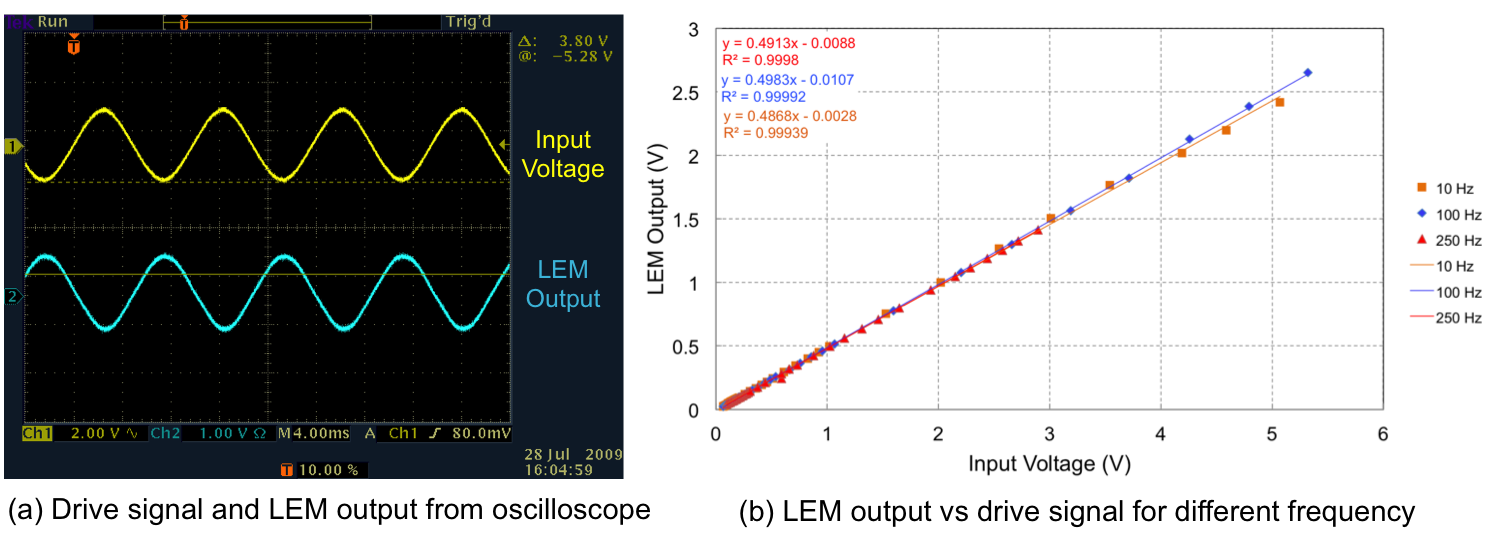
\includegraphics[width=15.0cm]{figures/BModLEMCalibration}
	\end{center}
	\caption
	[LEM current transducer output response to input sine drive signal.]
	{LEM current transducer output response (blue) to input sine drive signal (yellow) seen by oscilloscope (left). The output from the LEM was out of phase with the input signal. The figure on the right shows LEM calibration up to 5~V of input signal. The frequency dependence of the input signals were studied up to 250~Hz. The gains of the LEMs were $\sim$0.5.}
	\label{fig:BModLEMCalibration}
\end{figure}
\end{singlespace}


\subsection{LEM Current Transducer}
\label{LEM Current Transducer}
Four LEM CT-10T~\cite{LEM_CT-10T} were used to monitor the current through the two pairs of the MAT dipoles. %There was one spare LEM for backup. 
The LEM has two pins for the input current in one side and two power supply pins ($\pm$15~V) on the other side along with two pins for output voltages. The LEMs were calibrated up to 5.5~V of input voltage, whereas nominal input operating voltage during the experiment was $\sim$1~V. The calibration was performed using a bench top and VME-4145 signal generators. A typical drive signal and its readback signal by a LEM are shown in Figure~\ref{fig:BModLEMCalibration} (a) and the variation of LEM output with input drive voltage has been shown in Figure~\ref{fig:BModLEMCalibration} (b). There was a 180\degrees{} phase shift between the input (or Trim) signal and the LEM output signal. The measured gain was $\sim$0.5 for all the LEMs. There was no frequency dependence of the gain for the LEMs in the voltage domain 0 - 5~V as shown in Figure~\ref{fig:BModLEMCalibration} (b). The LEMs were assembled in an insulated box and installed in the Hall-C patch panel VME crate in the BSY service building~\cite{philip_communication} and were connected in series with the MAT dipoles. During the experiment, there was -75~mV, 240~Hz square wave noise injection in the beamline due to the cable connection fault in the LEM chassis. So, LEMs were disconnected during most of the production data taking. They were only turned on for tests and calibration during the commissioning period of the experiment. During preliminary bench test, LEM LA 50-P current transducer~\cite{LEM_LA_55-P} was used to monitor the current. LEM LA 50-P used the induction method to measure the current; hence there was no series connection with the coils for the measurements. Use of the induction current transducer has a lesser chance of injecting noise in the system. For future work, one might consider LEM LA 50-P or similar current transducer for precision parity measurements. The LEM current transducers have also helped to calibrate the strength of the magnets during the commissioning tests. More details about LEMs and its calibration are described in~\cite{nur_bm_lem}.

\subsection{Energy Modulation Hardware}
\label{Energy Modulation Hardware}
A 125~Hz sinusoidal signal was sent to an energy vernier SL-20 of a cryo-module in South linac of the accelerator to modulate the energy.
%This procedure uses an energy vernier SL-20 of a cryo-module in South Linac of the accelerator. Every 1~hour of a production run, the procedure will begin what is called a supercycle for $\sim$1~minute. Within each supercycle, modulation coil pair has its current ramped up and down with a proper ratio to each other. The final cycle of the supercycle is the modulation of the energy vernier. Each cycle can be programmed to be about 1~minute. The response of the beam position monitors and detectors can be measured. 
One of the standard features of the accelerator is the use of Fast Feed Back (FFB) system (Section~\ref{Fast Feed Back}) to maintain a steady beam position. 
Unfortunately, the energy FFB system did a perfect job of countering the 125 Hz energy modulation signal. 
The energy monitor BPM 3C12$X$ saw no response in Figure~\ref{fig:FFBEnergy} (bottom) for the energy modulation signal (top) when the FFB was on. 
%The times when the modulation signal was present (top) and the BPM 3C12X (energy monitor) response seen (bottom).  as in Figure.
So, the FFB system had been paused during the energy modulation to avoid any suppression from the FFB system. 
%
%Josh did a test last evening (in runs 15407 and 15408) in which he ran the energy modulation part of the BMod, but did not "pause" the FFB (i.e. in particular, no pause in the energy lock). This was to see if we can actually still modulate the beam energy with the system without pausing the fast feedback (since that pause seems to take a while to recover, and adds energy and position jitter to the beam before it comes back on).
%

%
%Not unexpected, and perhaps the response would be different at a different modulation frequency, but not promising way to go.
%
%A few things happen when we modulate. First there is a flexIO board in the trigger supervisor. It is used to send a pulse when we are ready to modulate. The signal/trigger is sent and the modulation runs for 4 seconds (511 cycles / 125 Hz) then stops. The board does not run continuously, it has a discrete number of cycles and then stops. After the four seconds the trigger is turned off, meaning we cannot trigger anymore regardless of what is shown anywhere else there will not be a trigger to the coils. In essence the change I made today won't change much if anything because by the time the trigger states of the boards are being changed the flexIO has been off for sometime. Paul correct me if I am wrong.

\begin{singlespace}
\begin{figure}[!h]
	\begin{center}
	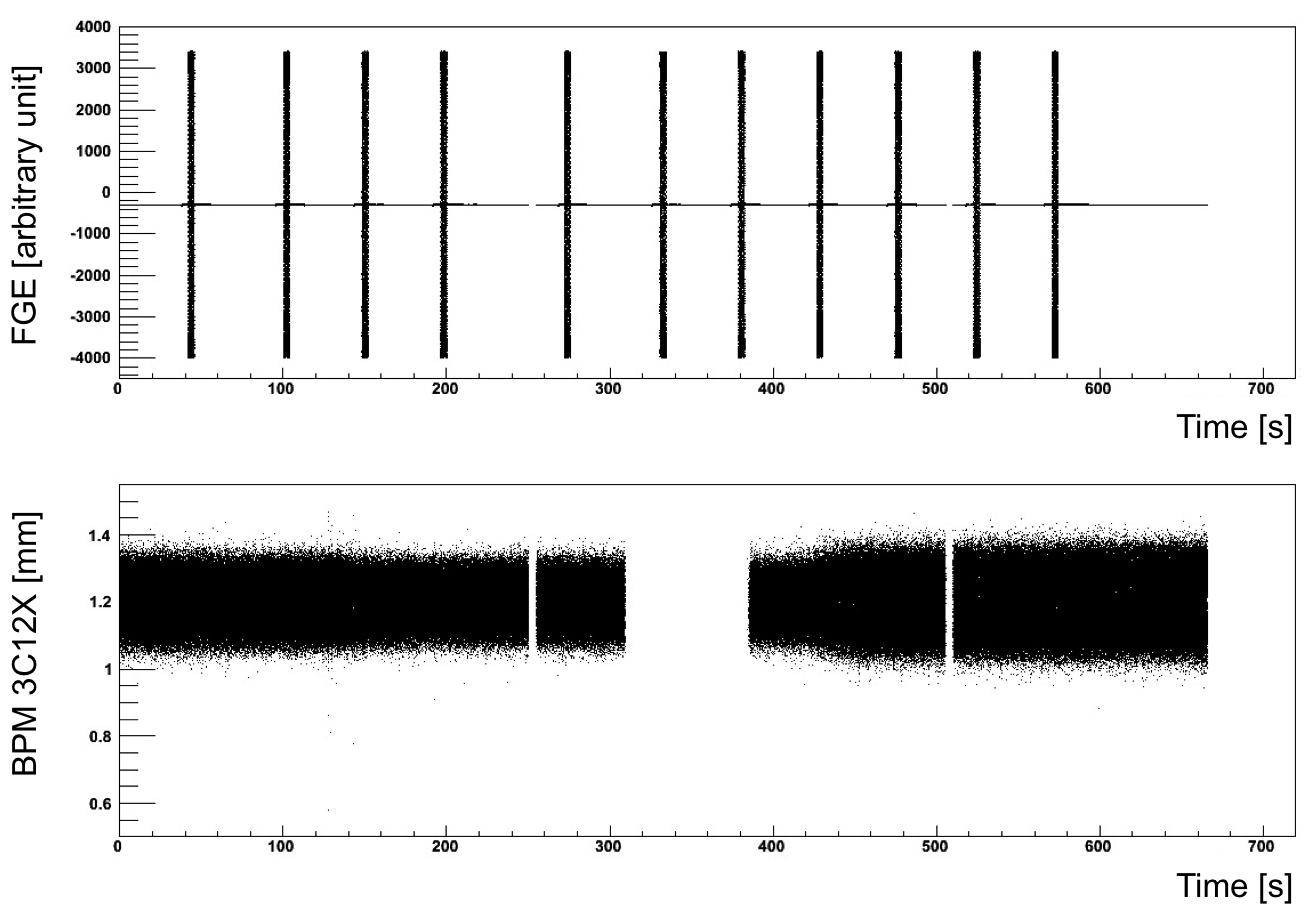
\includegraphics[width=10.0cm]{figures/FFBEnergy}
	\end{center}
	\caption
	[The effect of Fast Feed Back (FFB) system on energy modulation.]
	{The effect of Fast Feed Back (FFB) system on energy modulation~\cite{hclog:armd_249809}. Top panel shows function generator drive signal vs time. Bottom panel shows the response of the BPM 3C12$X$ (which is located in the middle of the arc and supposed to see maximum response for energy modulation) for the same drive signals. No response was observed in the BPM when FFB was on. The missing portions of the BPM response was removed by the software stability cut in order to avoid beam trips.}
	\label{fig:FFBEnergy}
\end{figure}
\end{singlespace}

\subsection{ADCs}
\label{ADCs}
Two sets of \newnot{symbol:TRIUMF}TRIUMF-built 18-bit analog to digital converters (\newnot{symbol:ADC}ADCs\index{ADC}) were used to study the readback signals from different components of the beam modulation system. 
%Two \newnot{symbol:TRIUMF}TRIUMF built 18-bit ADCs were used as main readback system. 
Each module had eight ADC channels which were synchronized and triggered by the MPS signal sent by the helicity board.
%(more details provided on TRIUMF ADCs in Section~\ref{Low Noise Electronics}). 
The ramp wave and 5 drive signals ($X$, $X^{\prime}$, $Y$, $Y^{\prime}$, $E$) from VME function generator, 4 readback signals from LEM current transducer, 4 readback signals from Trim-II power amplifiers were read by the TRIUMF ADCs (more details in section~\ref{Low Noise Electronics} and~\cite{website:TRIUMF, manual_TRIUMF_ADC} ). 

All the readback channels (above mentioned 14 channels and a readback from SL-20 vernier for energy modulation) were also sent to a 32-channel JLab made ADC module~\cite{JLab_ADC} which was used to monitor the peaks of the signals.
%Another JLab made a 32-channel ADC module~\cite{JLab_ADC} was used to monitor the peaks of the 5 drive signals, 4 readback signals from LEM current transducer, and 4 readback signals from Trim-II power amplifiers. 
The ADC had 16-bit resolution and supported up to a 100~kHz sample rate. The ADC was configured by 36 16-bit registers and read the analog input data. The data format was configured depending on the selected bipolar or unipolar input range. The analog inputs were fully differential and configured to detect the peak of the input signals. The input connectors for the analog inputs were 50-pin D style connectors. The front panel had indicator LED's for power and heartbeat. 
%The idea behind JLab peak detection ADC was to have a standalone (independent of Q-weak parity violating data acquisition system) modulation readback system. 
The JLab-made peak detection ADC was used as a standalone (independent of Q-weak parity violating data acquisition system) modulation readback system and was installed in the BSY service building.

%\begin{singlespace}
%\begin{table}
%\begin{center}
%  \begin{tabular}{| c | c |}
%    \hline
%    	The Components & Quantity \\ \hline
%			Signal Generator & 1 \\ \hline
%			TRIM-II & 2 \\ \hline
%			MAT Coil & 2 \\ \hline
%			LEM & 1 \\ \hline
%			Ammeter & 2 \\ \hline
%			Power Supply & 1 \\ \hline
%			Tesla Meter & 1 \\ \hline
%  	\end{tabular}
%  	\caption[Beam modulation bench test]{Beam modulation bench test}
%  \label{bench_test}
%\end{center}
%\end{table}
%\end{singlespace}

\begin{singlespace}
\begin{figure}[!h]
	\begin{center}
	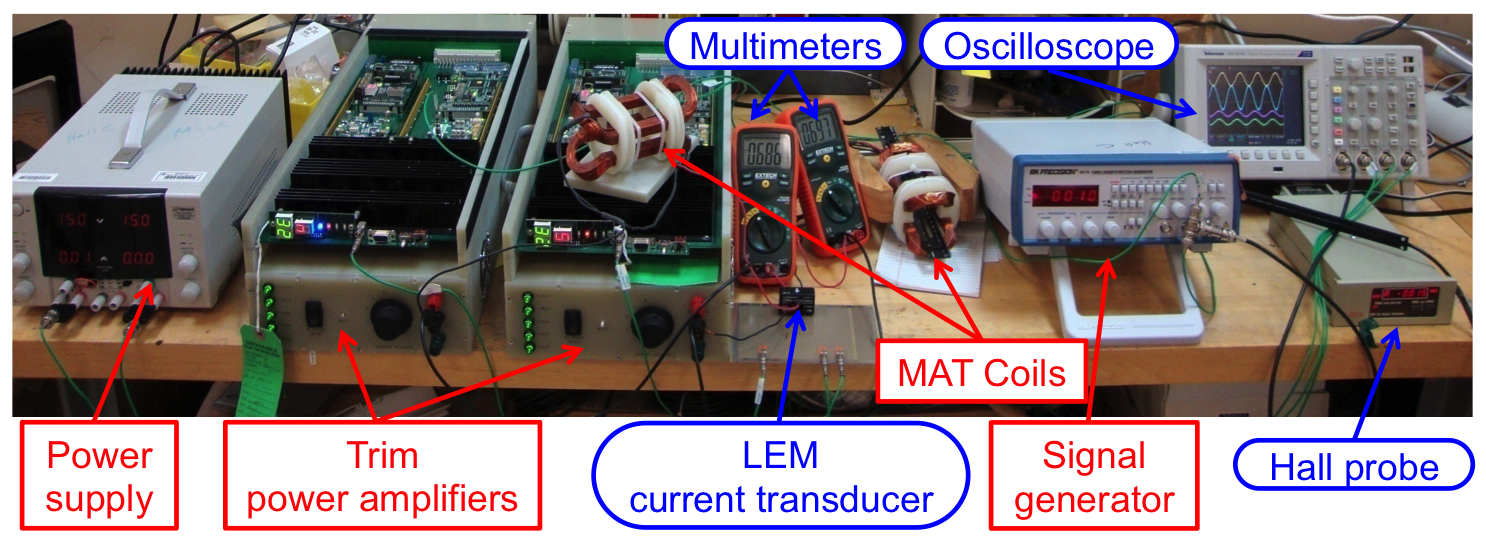
\includegraphics[width=15.0cm]{figures/BModTestHardware}
	\end{center}
	\caption
	[Beam modulation hardware bench test setup.]
	{Beam modulation hardware bench test setup. It consists of one $\pm$15~V power supply, two Trim power amplifiers, pair of assembled MAT coils, and one signal generator. A VME signal generator was also used during the latter part. To see the responses and read-backs, two multimeters, a LEM current transducer, a hall probe, and an oscilloscope were used. }
	\label{fig:BModTestHardware}
\end{figure}
\end{singlespace}

%%%%%%%%%%%%%%%%%%%%%%%%%%%%%%%%%%%%%%%%%%%%%%%%%%%%%%%%%%%%%%
%\section{Bench Tests}
%\label{Bench Tests}
%Extensive bench tests were performed with the beam modulation system so that (except for the absence of long drive cables) it would be possible to predict how the installed system would work. The Trim amplifier was controlled via an analog input from a simple bench-top function generator at the beginning and latter with VME 4145 board. 
%The signal generator produces sine wave of different amplitude and frequency as the input voltage to the Trim-II power amplifier. The amplified signal goes to $\sim$10~cm long MAT coil through a single LEM current transducer either in phase or out of phase from two coils. The currents through the coils were measured by ammeter. The magnetic fields of the coils were measured by the Tesla meter. All the individual components were tested and calibrated in the bench test. The bench test setup is shown in Figure~\ref{fig:BModTestHardware}.
%
%
%%\begin{singlespace}
%%\begin{figure}[!h]
%%	\begin{center}
%%	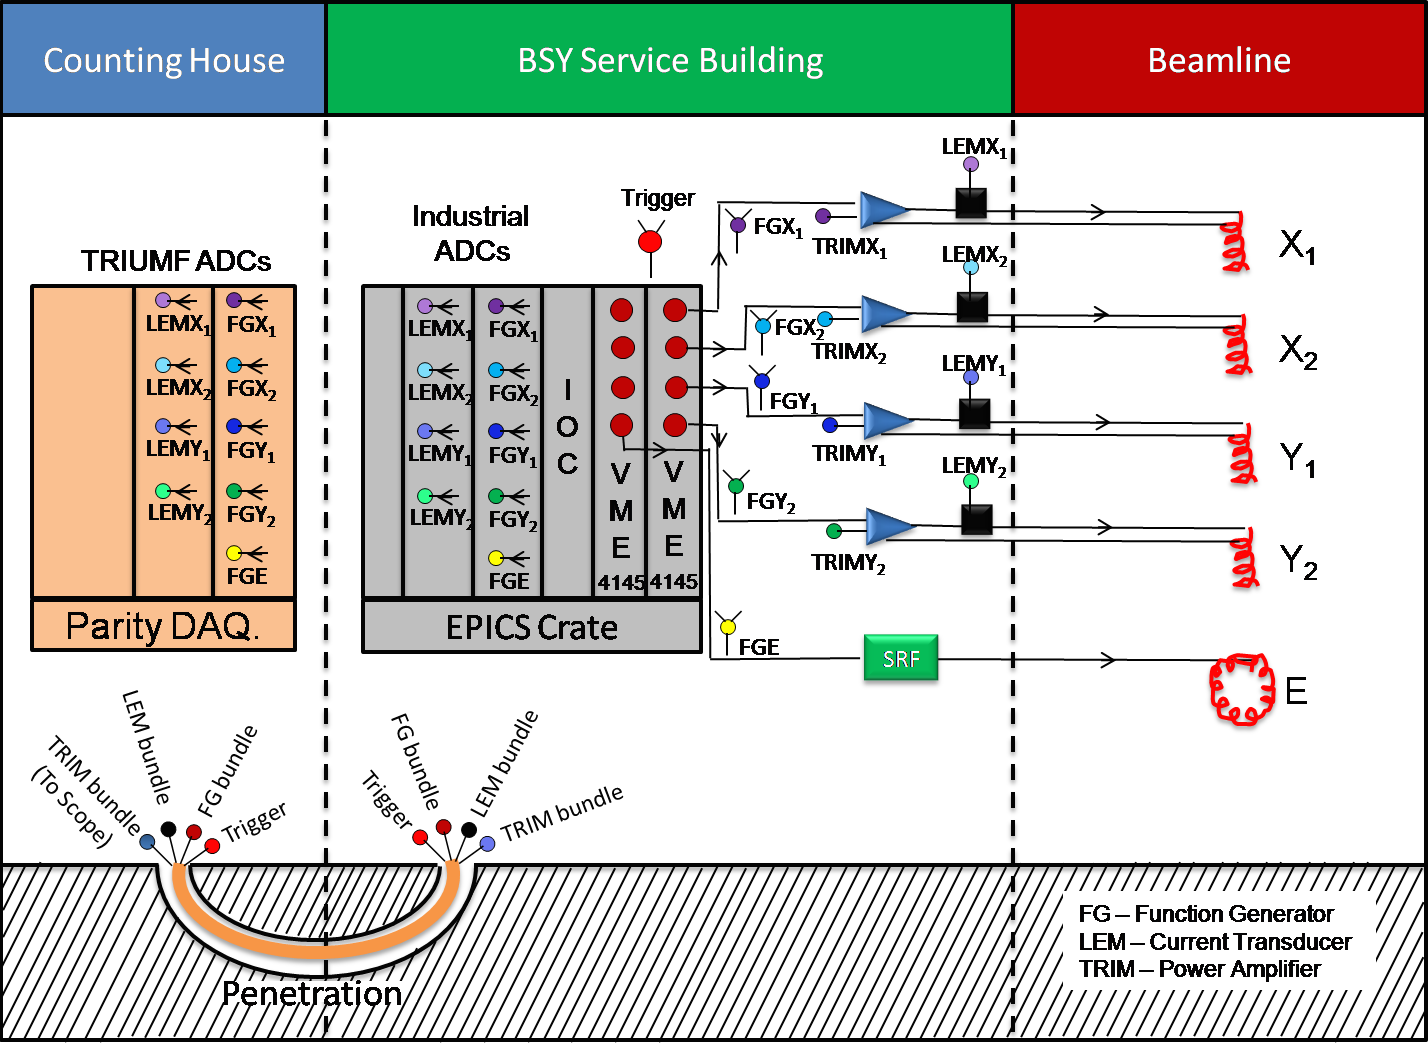
\includegraphics[width=15.0cm]{figures/BModCable}
%%	\end{center}
%%	\caption[Beam modulation cable sketch.]{Beam modulation cable sketch.}
%%	\label{fig:BModCable}
%%\end{figure}
%%\end{singlespace}

%%%%%%%%%%%%%%%%%%%%%%%%%%%%%%%%%%%%%%%%%%%%%%%%%%%%%%%%%%%%%
\section{Hardware Components Calibration and Important Constraints}
\label{Hardware Components Calibration and Important Constraints}
Extensive bench tests were performed with the beam modulation system so that (except for the absence of long drive cables) it would be possible to predict how the installed system would work. The Trim amplifier was controlled via an analog input from a simple bench-top function generator at the beginning and latter with VME 4145 board. 
The signal generator produces sine waves of different amplitudes and frequencies as the input voltage to the Trim-II power amplifier. The amplified signal goes to $\sim$10~cm long MAT coil through a single LEM current transducer either in phase or out of phase from two coils. The currents through the coils were measured by ammeter. The magnetic fields of the coils were measured by the Tesla meter. All the individual components were tested and calibrated in the bench test. The bench test setup is shown in Figure~\ref{fig:BModTestHardware}.

\subsection{Coil Positioning}
\label{Coil Positioning}
There were significant constraints on where perturbing coils could be located. One absolute requirement was that coils be located upstream of the high dispersion point at 3C12 (the center of the 3C arc) so that modulations in $X$, $X^{\prime}$, and $E$ could be disentangled. Another highly desirable constraint was that the coils be located downstream of any expected deviations from design optics. Accelerator operations agreed to complete matching in 3C beamline by quadrupole MQA3C08, the beginning of the 3C arc dipole string. Considerations of robustness and purity therefore excluded regions upstream of this point, leaving only only the first half of the 3C arc as a potential site for coils. 
This coil positioning and orbit excursions were simulated using OptiM. Initially, it was attempted to insert both coils into a single $\sim$1~m drift, but the angle kicks of interest required excessively high field integrals and the approach did not work. Separating the coils by more than 1 meter required straddling other beamline elements. The coils were mounted between two dipoles (since the orbit inside a dipole is plotted effectively like a drift) with no intervening quadrupoles or active elements between them. The 1st pair of MAT coils, MHF3C08H ($X_{1}$) and MHF3C08V ($Y_{1}$), were installed in the drift oD7028, which was located just after quadruple 3C08 and before the dipole 3C05. The 2nd pair MAT coils, MHF3C10H ($X_{2}$) and MHF3C10V ($Y_{2}$), were installed in the drift 0D7034, which was located between dipoles 3C06 and 3C07. The separation between these two pairs of coils was about $\sim$9.5~m. The first coil $X_{1}$ was located $\sim$92.7~m upstream of the Q-weak target.  %The two pairs of coils had opposite polarity, 1st pair kick the beam in o and deflected the beam in .
The $X_{1}$ and $X_{2}$ coils were pulsed at a time and in opposite phase to produce relatively pure horizontal position or angle changes at the target, for virtually any tune of the beamline as shown in Figure~\ref{fig:BModDrawing}.

%The used nomenclature was from the OptiM deck found in Appendix II. As shown in Figure 5, our 1st coil is in drift oD7028, located just after quadruple 3C08 and before the dipole 3C05. The 2nd coil will be in drift 0D7031, after dipole 3C06 but before dipole 3C07. The separation is about 9.5 m. 

\subsection{Waveform}
\label{Waveform}
The Trim power amplifier was unable to drive square or even triangular waveforms in the frequency range of interest. Satisfactory results were obtained only with sinusoidal waveform, which was hence was used to drive the magnets. The preferred waveform was to generate at least square-ish modulation (similar to the square helicity reversal) and needed different power amplifier. Due to budget and schedule pressure, existing Trim amplifiers were used.

\subsection{Waveform Phase}
\label{Waveform Phase}
A 1~V of sawtooth wave with the same frequency of 125~Hz as sinusoidal drive signal from VME 4145 was used to monitor the phase of the drive signals. The sawtooth ramp wave goes from 0 to 1~V as the phase of the sinusoidal drive signal goes from 0 to 360$^{o}$ (Figure~\ref{fig:BModSignalZoomed}). The drive signal and ramp wave were triggered together to match and lock the phase. The edges of the ramp wave were not very sharp hence were removed during the analysis to avoid any edge effect. The edges were recreated using a ramp fill method in the software as described in~\cite{elog:don_analysis948}. 

\begin{singlespace}
\begin{figure}[!h]
	\begin{center}
	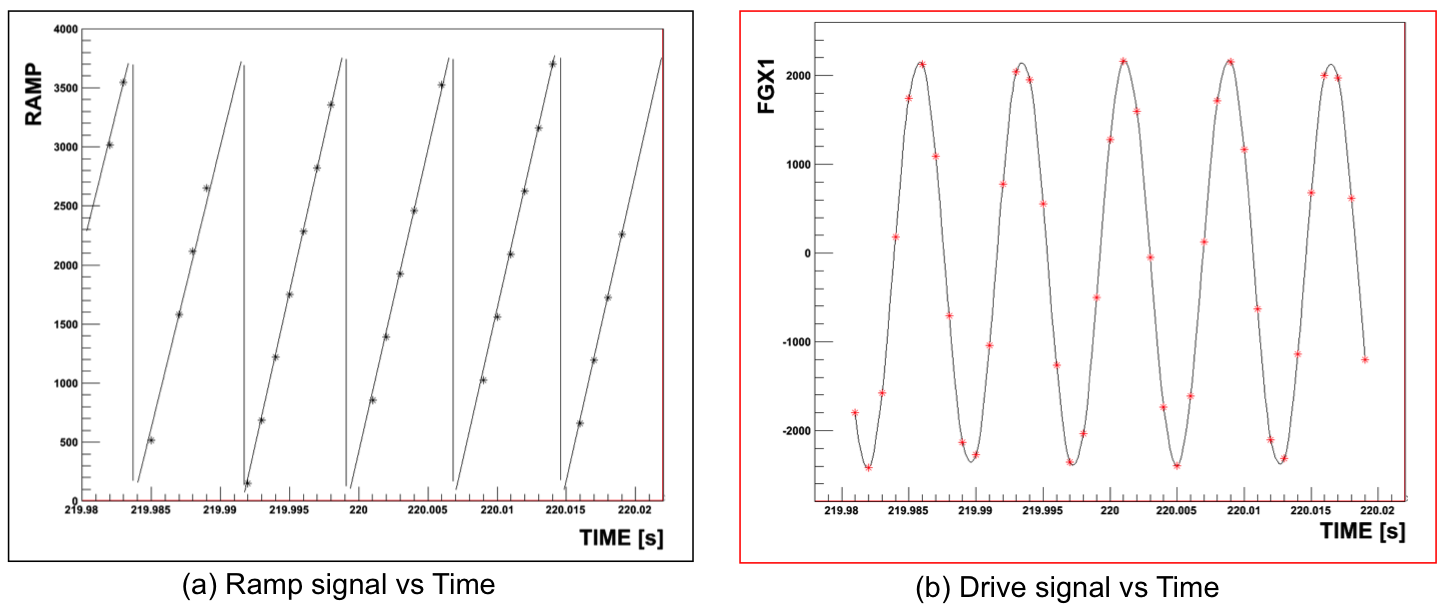
\includegraphics[width=15.0cm]{figures/BModSignalZoomed}
	\end{center}
	\caption
	[Zoomed ramp and drive signal from a beam modulation cycle during a typical production run.]
	{Zoomed ramp and drive signal from a beam modulation cycle during a typical production run. (a) Ramp signal vs time. The ramp signal is a sawtooth wave used to track the phase of the other sinusoidal drive signals. (b) Drive signal vs time. The drive signal is a sinusoidal wave with fixed phase. }
	\label{fig:BModSignalZoomed}
\end{figure}
\end{singlespace}


\subsection{Frequency Range}
\label{Frequency Range}
The frequency of the waveform was tested for the range of 10-500~Hz and nominal 3~A (peak) output. The Trim cards reliably drove sinusoidal waveforms up to 250~Hz. At that frequency, the coil impedance becomes approximately $X_\textrm{total}$ = 1.6~$\Omega$ + 2$\pi f$ (0.0038~H) = 7.6~$\Omega$, so the amplifier has to provide 22.8~V (peak). The maximum output voltage of the Trim-II amplifier appeared to be approximately $\pm$~27~V, but it was not strictly bipolar due to the use of NPN diodes for one polarity and PNP diodes for the other. So while one could go a bit higher in frequency than 250~Hz, there would be a rapidly increasing risk of generating asymmetrical sine-like waves (and hence a small DC beam position offset). During production data collection, the nominal drive signal frequency was 125~Hz to stay inside the linear region of the Trim operation. Another criteria for choosing the frequency was to avoid the power line frequencies (60, 120, 180, etc.~Hz) suppressed by FFB system.

\subsection{Maximum Current}
\label{Maximum Current}
With sustained operation, the coils became quite hot to the touch at $I_\textrm{peak}$ = 7.07~A ($I_\textrm{rms}$ = 5~A). This was significantly above Q-weak's nominal maximum current $I_\textrm{peak}$ = 3~A, but it is worth discussing since future experiments at higher beam energy might try to push the envelope. Although measurements at 1\% duty factor would take only 36~seconds per hour, one must assume that a parity violation experiment will eventually take long, dedicated beam modulation runs. Unless cooling fans installed, damage to the enamel-insulated wires or any plastic components could result if $I_\textrm{peak}$ = 7.07~A is significantly exceeded. The ``smoke point" of the magnets was not determined, but bear in mind that $P$ = $I^{2}R$, so the temperature would increase rapidly with current above $I_\textrm{peak}$ = 7.07~A. It is hopefully understood that $I_\textrm{peak}$  = 7.07~A refers to the peak current of a sinusoidal waveform, and not to a maximum DC current which would have twice the power dissipation. Constraint on maximum current based on machine protection simulation is discussed in the Section~\ref{Machine Protection Analysis}.
 
 \begin{singlespace}
\begin{figure}[!h]
	\begin{center}
	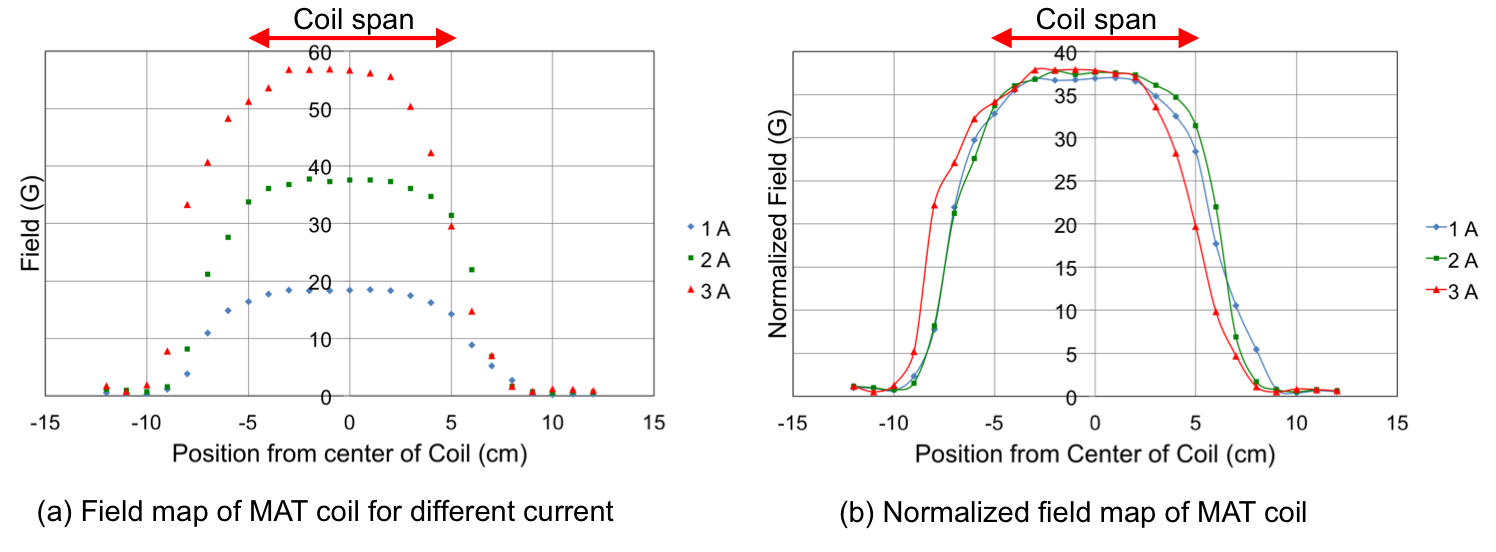
\includegraphics[width=15.0cm]{figures/BModMATFieldIntegral}
	\end{center}
	\caption
	[Field map of MAT coil for different input coil currents.]
	{Field map of MAT coil for different input coil currents (left). The filed was linear in the region of the coil span of 10~cm. The field profile did not change with coil current upto 3~A. The field was normalized with respect to 1~A (right).}
	\label{fig:BModMATFieldIntegral}
\end{figure}
\end{singlespace}

\subsection{Magnetic Field Calibration of the MAT Coils}
\label{Magnetic Field Calibration of the MAT Coils}
The MAT coils were calibrated using a bench test setup, as shown in Figure~\ref{fig:BModTestHardware}. The magnetic field was measured using a GMW Hall Probe. The measured field integral for 10~cm MAT coil was $\sim$330~G-cm/A. The field was reasonably stable for the span of the coil (Figure~\ref{fig:BModMATFieldIntegral} (a)). There was no current dependence of the field as shown in Figure~\ref{fig:BModMATFieldIntegral} (b). The magnetic field for the MAT coils falls quite sharply with distance beyond the coil span, hence reduces the possibility of interaction with other active elements in the beamline.

%\section{Observations}
%\label{Observations}
%The TRIM II is not a linear device. It has frequency dependence. As we are going to higher frequencies starting from 10 Hz to 500 Hz, we are getting higher output voltages across the coils for same input voltage form signal generator with sine wave. As we are going to higher voltages for a fixed frequency, the TRIM II is showing non linearity also. Near the saturation current the TRIM II is getting locked by itself especially with higher frequency. 
%We are a getting a phase shift of 180� between the TRIM II output and the LEM current. 
%

%%%%%%%%%%%%%%%%%%%%%%%%%%%%%%%%%%%%%%%%%%%%%%%%%%%%%%%%%%%%%
\section{Controls and Software Sketch}
\label{Controls and Software Sketch}
A standalone control system for the beam modulation system was designed by Scott Higgins~\cite{nur_bm_controls, higgins_communication, nur_bm_GUI_proposal}. 
The drive signals of two VME-4145 signal generator boards was controlled via an EPICS database access library that works on Unix and vxWorks. 
In the control system, the first VME-4145 card was referred as ${\tt BMOD1}$ and the second card as ${\tt BMOD2}$. Each function generator card has 4 channels and they are named as ${\tt CHAN0}$, ${\tt CHAN1}$, ${\tt CHAN2}$, and ${\tt CHAN3}$. All four channels of ${\tt BMOD1}$ and ${\tt CHAN0}$ and ${\tt CHAN3}$ of ${\tt BMOD2}$ were used for the modulation system. 
The EPICS variable for the master switch was ${\tt BEAMMODSWITCH}$. A value for ${\tt BEAMMODSWITCH}$ of 0 was considered as ${\tt OFF}$ and 1 was ${\tt ON}$.  This switch allowed operations to control whether or not to allow any beam modulation requests. The off state was entered when the master switch was set to ${\tt OFF}$. In the ${\tt OFF}$ state the Relays to the Trim cards were set to ground. The ${\tt OFF}$ state was the default state for the system after an IOC reboot. The ${\tt CONFIG}$ state was entered when the operations toggles the master switch from ${\tt OFF}$ to ${\tt ON}$. Once the board was in the ${\tt CONFIG}$ state all, the channels in ${\tt BMOD1}$ and one channel ${\tt BMOD2}$ were allowed to load a sine wave, whereas ${\tt CHAN0}$ of ${\tt BMOD2}$ was allowed to load ramp wave. The inputs controlling the sine wave were frequency and amplitude. The allowed frequency range was set to be 10-250~Hz, and amplitude was limited to $\pm$~0.3~A, as discussed in previous sections. A negative amplitude would shift the phase of the sine wave by 180\degrees{}/$\pi$. The amplitude output for ramp wave was between 0 and 1~V. The ramp wave period started at 0~volt and then the slope linearly increased to the amplitude entered. Then the ramp wave was loaded the same way as other drive signals. Before the transitions to the trigger state, it was necessary to enter the number of periods for the sinewave or rampwave to run the system. This setting ranged from 1 to 511. A value of 511 would cause the hardware to run the sinewave or rampwave continuously which was a feature of the hardware. Nominal cycle for the system was set to 510. The trigger state was entered by writing a value of 1 to the EPICS variable ${\tt TRIGGER}$ state.
%, then the following took place transitioning from the ${\tt CONFIG}$ state to the ${\tt TRIGGER}$ state:
%
%\begin{itemize}
%	\item A single period of the sine wave was run to force a value of zero on the output of the Function Generator.
%	\item The software waits 1~second to make sure the zeroing occurred. This value was found empirically and is usually long enough. There is a chance that the single period of the sine wave will run after the relay is engaged.
%	\item The relay for this channel is enabled. The function generator output is connected to the Trim card.
%	\item The software verifies that the relays are enabled and goes to the ${\tt TRIGGER}$ state.
%\end{itemize}

The sine waves could be initiated by both a hardware and software trigger. The software trigger was a button that is activated by writing a value of ``1" to the EPICS variable. This feature was primarily used in testing the system. The hardware trigger was initiated from the Hall-C parity violating DAQ. All of the 8 channels shared the same hardware trigger so any of the channels that were in the ${\tt TRIGGER}$ state would initiate sine wave outputs. It should be noted that if another trigger comes in while the VME-4145 is outputing a sine wave, the output will be interrupted and the card will restart the sine wave from the beginning. There were 2 things that could cause a channel to leave the trigger state: if operations selects Beam Modulation Off with the master switch or the user selects to leave the trigger state. The EPICS variables to leave the trigger state is activated by writing a value of ``1". 
%The following took place transitioning from the trigger state to the ${\tt CONFIG}$ state.
%
%\begin{itemize}
%	\item Relays were commanded open for the channel.
%	\item VME-4145 channels were commanded to stop producing sine wave.
%	\item Software verifies that the relays were open and once confirmed goes to the ${\tt CONFIG}$ state.
%\end{itemize}

If the user entered the trigger state after having previously run a sinewave, the last loaded sine wave would be executed. There was no need to reload the sine wave in the ${\tt CONFIG}$ state if amplitude and frequency were to stay the same. If, however, the user desired to change either the frequency or amplitude, a new sinewave must be loaded. There was a time delay in the reporting of the running of a sinewave from the VME-4145. A sine wave could be triggered and finished before the card reported that it was actively running a sinewave. Therefore there was no deterministic way to see the status of the card generating a wave for a particular channel in real time, at least not by monitoring the VME-4145. An external method was needed. A JLab-made ADC was used to monitor those channels in real time. There was a signal that went back to the hall which showed the output of the VME-4145 function generator. The goal of this signal was to show real time values written to the trim card. In order for the output of the function generator to reach the trim card, a relay needed to be set. The signal going back to the Hall-C of the function generator was between the relay board and the trim card. There were 2 RELAYS for each VME-4145 function generator channel. Both were set for the channel to be connected the trim card. A value of ``1" meant the relay was enabled and the function generator was connected to the trim card. A value of ``0" meant the relay was off and the trim card was tied to ground. More details about the modulation control system can be found in technical documents~\cite{nur_bm_controls, nur_bm_GUI_proposal}.


%%%%%%%%%%%%%%%%%%%%%%%%%%%%%%%%%%%%%%%%%%%%%%%%%%%%%%%%%%%%%
\section{Modulation Modes}
\label{Modulation Modes}
Two possible modulation modes were exercised during the experiment. One mode was with single coil modulation, where all four coils $X_{1}$, $X_{2}$, $Y_{1}$, and $Y_{2}$ were pulsed individually; this mode was mainly used to calibrate and test the system during commissioning period. The other mode was, in which one pair of coils was pulsed together to achieve relatively pure position and angle at the target, was used as nominal mode for the modulation operation. A pulse with a combination of $X_{1}$, and $X_{2}$ was used for horizontal position and angle, and one with a combination of $Y_{1}$, and $Y_{2}$ was used for vertical position and angle motion. The energy modulation was the same for both the modes. The motivations for using a pair over a single dipole were greater flexibility in coil positioning, coil positions being independent of beamline optics, and a compact configuration. The nominal current through the MAT dipole for the pair mode is shown in Table~\ref{tab:beam_parameter}. A unique pattern number was assigned in the software to identify the different modulation modes, and parameters as listed in Table~\ref{tab:modulation_mode}.

\begin{singlespace}
\begin{table}[!h]
\begin{center}
  	\caption
	[Different beam modulation modes and related pattern numbers.]
  	{Different beam modulation modes and related pattern numbers. In single coil mode, just one coil was pulsed and the response was a linear combination of position and angle. In pair of coils, two coils were pulsed at a time to produce relatively pure position or angle.}
  \begin{tabular}{ c | c | c | c }
%    \hline
    \noalign{\hrule height 1pt}
    	Mode & Parameter	&	Coils Pulsed &	Pattern Number \\ 
%    	\hline
    \noalign{\hrule height 1pt}
    \multirow{5}{*}{Single coil} & $X$ and $X^{\prime}$		&	$X_{1}$	& 1 \\
     & $X$ and $X^{\prime}$		&	$X_{2}$	& 2 \\
     & $Y$ and $Y^{\prime}$		&	$Y_{1}$	& 3 \\
     & $Y$ and $Y^{\prime}$		&	$Y_{2}$	& 4 \\
     & $E$		&	E	& 5 \\
	\hline
%    \noalign{\hrule height 1pt}
    \multirow{5}{*}{Pair of coils} & X	&	$X_{1}$ and $X_{2}$	& 11 \\
     & $Y$		&	$Y_{1}$ and $Y_{2}$  & 12 \\
     & $E$		&	$E$  & 13 \\
     & $X^{\prime}$		&	$X_{1}$ and $X_{2}$  & 14 \\
     & $Y^{\prime}$		&	$Y_{1}$ and $Y_{2}$  & 15 \\
%	\hline
    \noalign{\hrule height 1pt}
  	\end{tabular}
  \label{tab:modulation_mode}
\end{center}
\end{table}
\end{singlespace}




\begin{singlespace}
\begin{figure}[!h]
	\begin{center}
	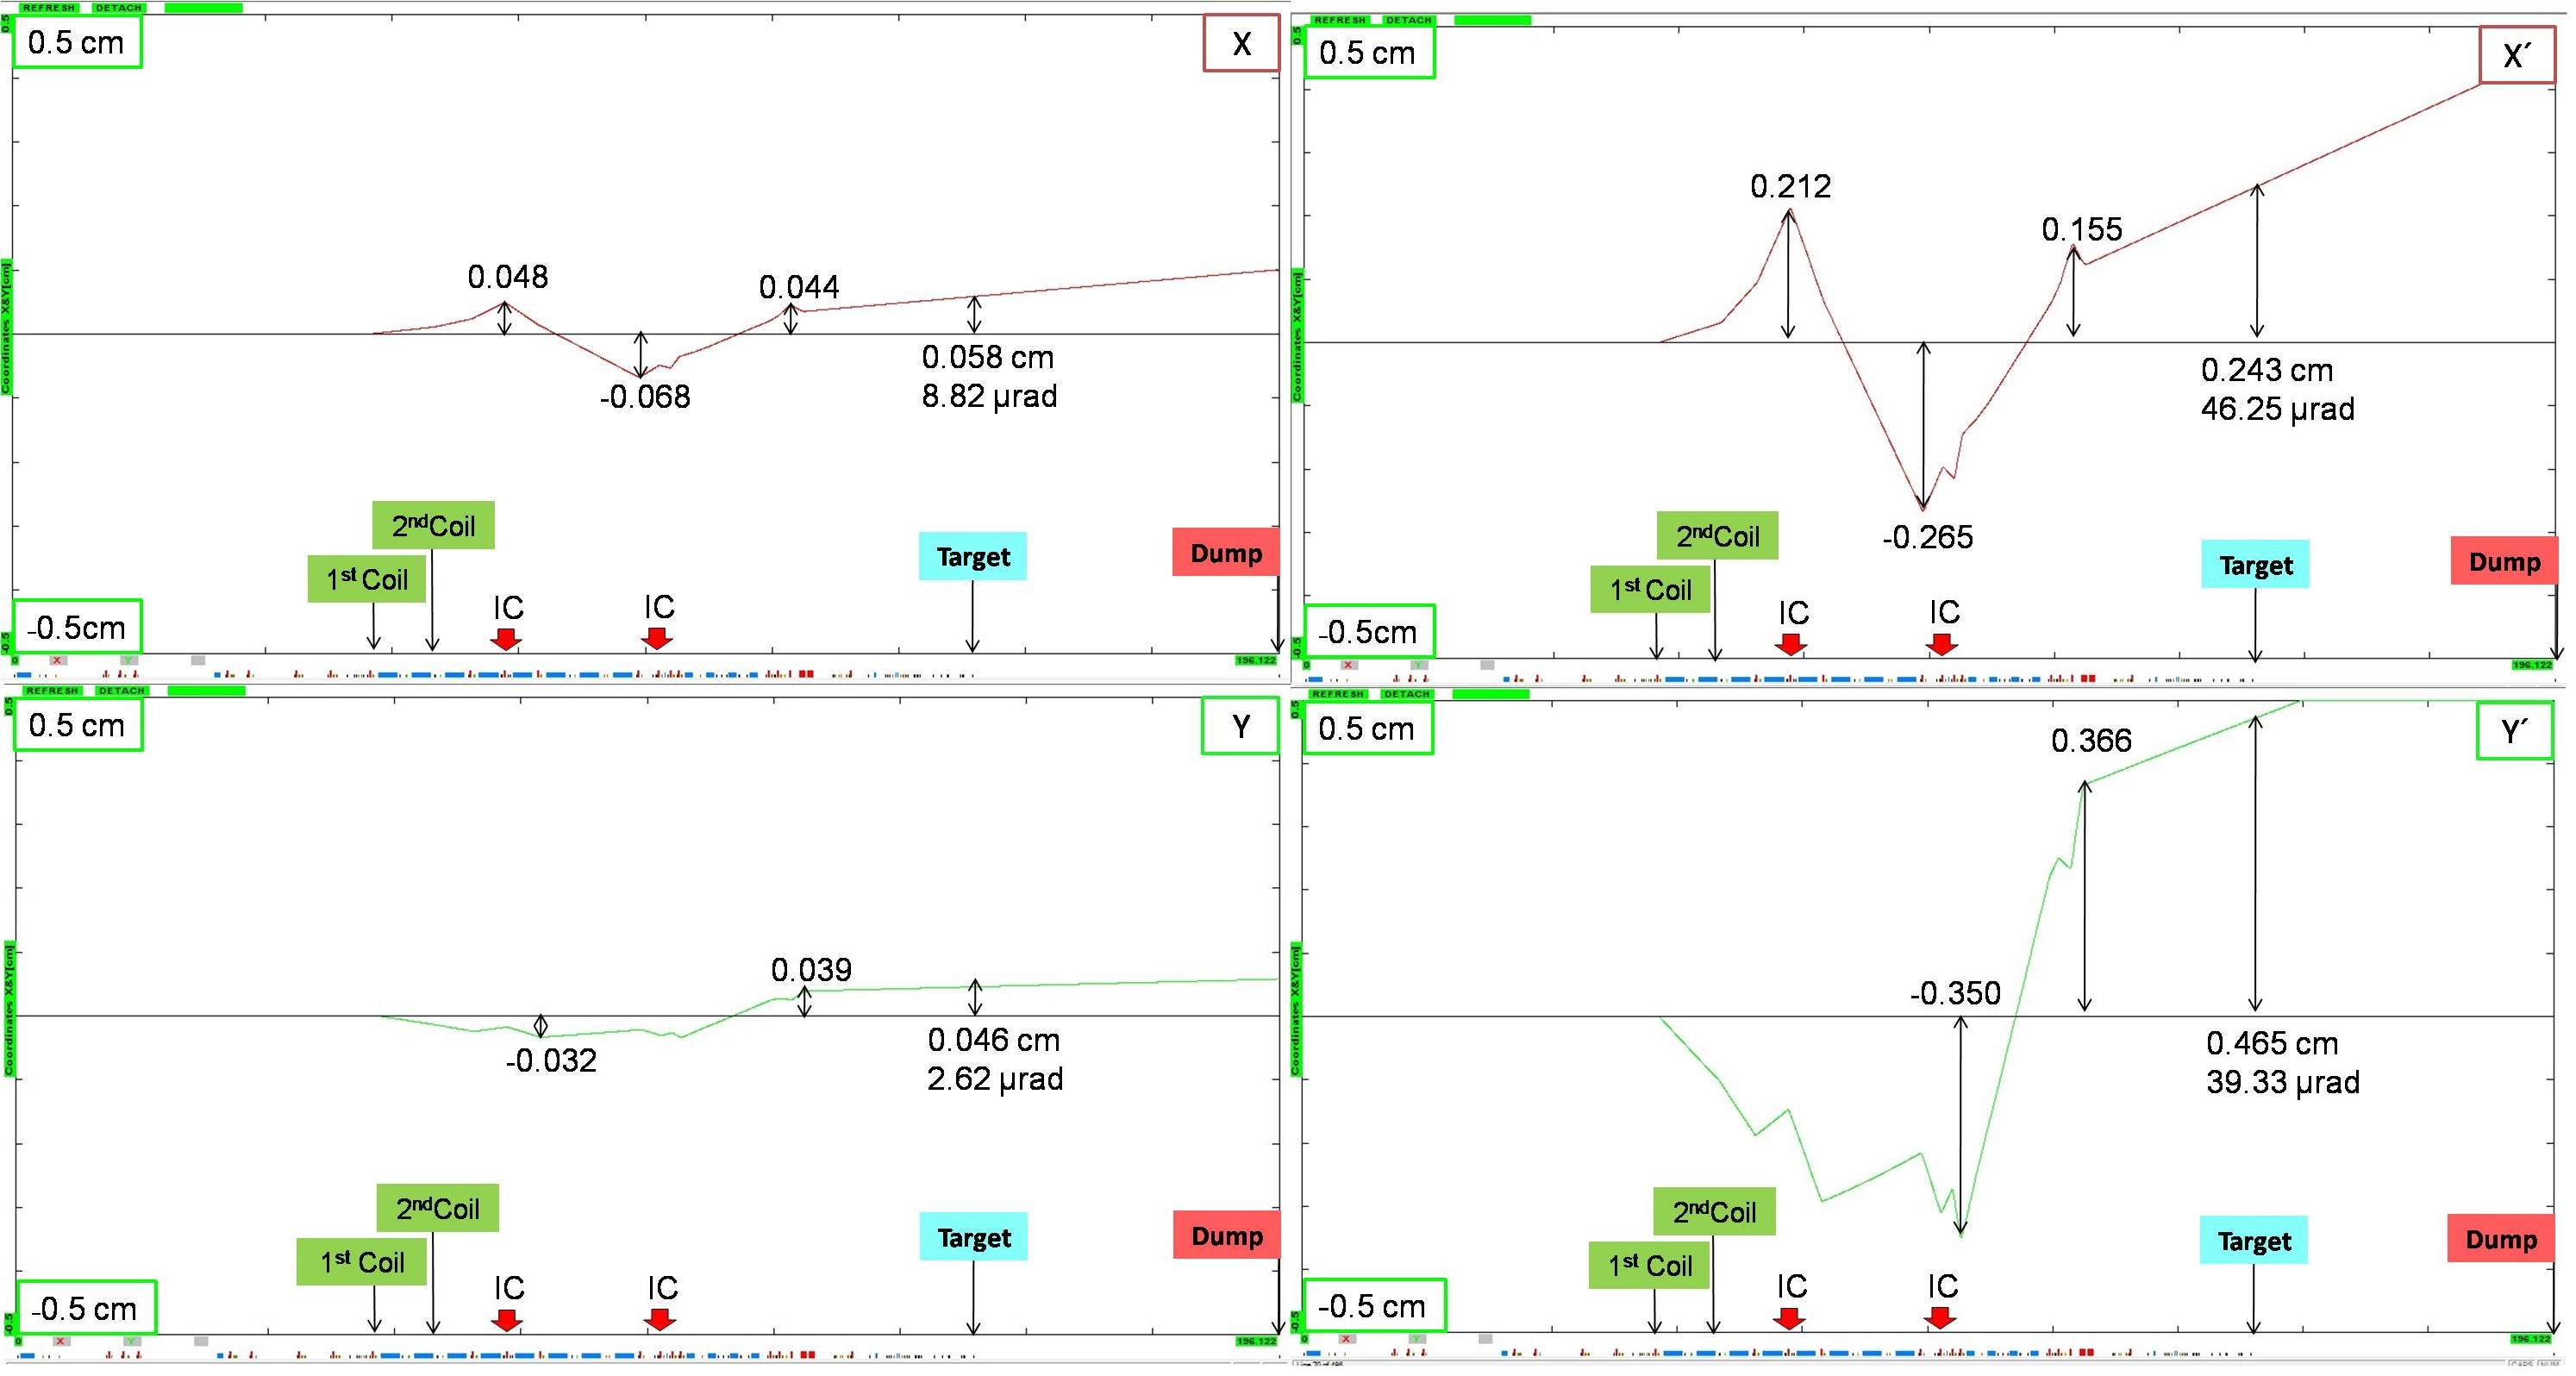
\includegraphics[width=15.0cm]{figures/BModMachineProtectionAllPair}
	\end{center}
	\caption
	[Orbit excursions using a pair of coils with incorrect polarity on one of the coil.]
	{Orbit excursions using a pair of coils with incorrect polarity on one of the coil. Beam moves from left to right. Large excursions were observed for angle compared to position. The used field strength to pulse the coils for this simulation was 5 times higher than that used as nominal field strength during the experiment. The location for ion chambers (IC) was recommended based on this study and is shown by the thick arrows at the bottom of the figure.}
	\label{fig:BModMachineProtectionAllPair}
\end{figure}
\end{singlespace}


%%%%%%%%%%%%%%%%%%%%%%%%%%%%%%%%%%%%%%%%%%%%%%%%%%%%%%%%%%%%%
\section{Machine Protection Analysis}
\label{Machine Protection Analysis}
A simulation was performed to check the maximum possible excursion in the beamline due to beam modulation magnet kicks. The nominal field integrals for the modulation MAT coils are given in Table~\ref{tab:beam_parameter} and the corresponding excursions are shown in Figure~\ref{fig:BModForwardBeamline}. For this simulation, the modulation kicks were increased by increasing the nominal field by 5 times to enhance the effect (these excursions are linearly scaled). The beam excursions with this conditions were 1.3~mm at the upstream of the target and 1.0~mm at the beam dump. The tune parameters in Table~\ref{tab:beam_parameter} were negative, which implies the opposite polarity of the magnets. To check the worst possible scenario, the polarity of the magnets was reversed (using the same 5 times of nominal field); the simulated orbits are shown in Figure~\ref{fig:BModMachineProtectionAllPair}. The reversed polarity deviations upstream of the target were 3.6~mm and 6.6~mm at the beam dump. The same simulation with only one coil energized deviations was 2.4~mm upstream of the target and 3.8~mm at the beam dump for $I_\textrm{max}$ = 0.6~A.
Considering all of these cases, the maximum obtained excursion was about 4.6~mm at the target for a maximum current of 0.6~A. For angles, the excursions were much larger than position excursion mainly in the regions middle of the arc (around quadrupole 3C12) and end of the arc (around quadrupole 3C17). The deviation at the beam dump was 6.6~mm for $I_\textrm{max}$ = 0.6~A.
For protection of the machine, considering all the above cases, the recommended place to install ion chambers (IC) was at the highest beam excursion region of the beamline around 3C12 and 3C17 (as shown in Figure~\ref{fig:BModMachineProtectionAllPair}). 
The worst case scenario was found to be the case of incorrect polarity. 
In order to avoid any mishap, when system was commissioned, a hard coded software limit of $I_\textrm{max}$ = 0.3~A was implemented for the safety of the accelerator. 
%This document shows that the beam excursions under nominal conditions are $\leq$ 1mm, under reversed polarity deviations can be 3.6 mm while only one coil energized deviations can be 2.4 mm for $I_{max}$ = 0.6 A. It also shows the excursion of beam for the case when the beam is pulsed by individual coils. It also talks about the regions of high excursions that need our attention for three unforeseen cases mentioned above.
More details about the machine protection analysis can be found in Q-weak internal technical document~\cite{nur_bm_machine_protection}.

\begin{singlespace}
\begin{figure}[!h]
	\begin{center}
	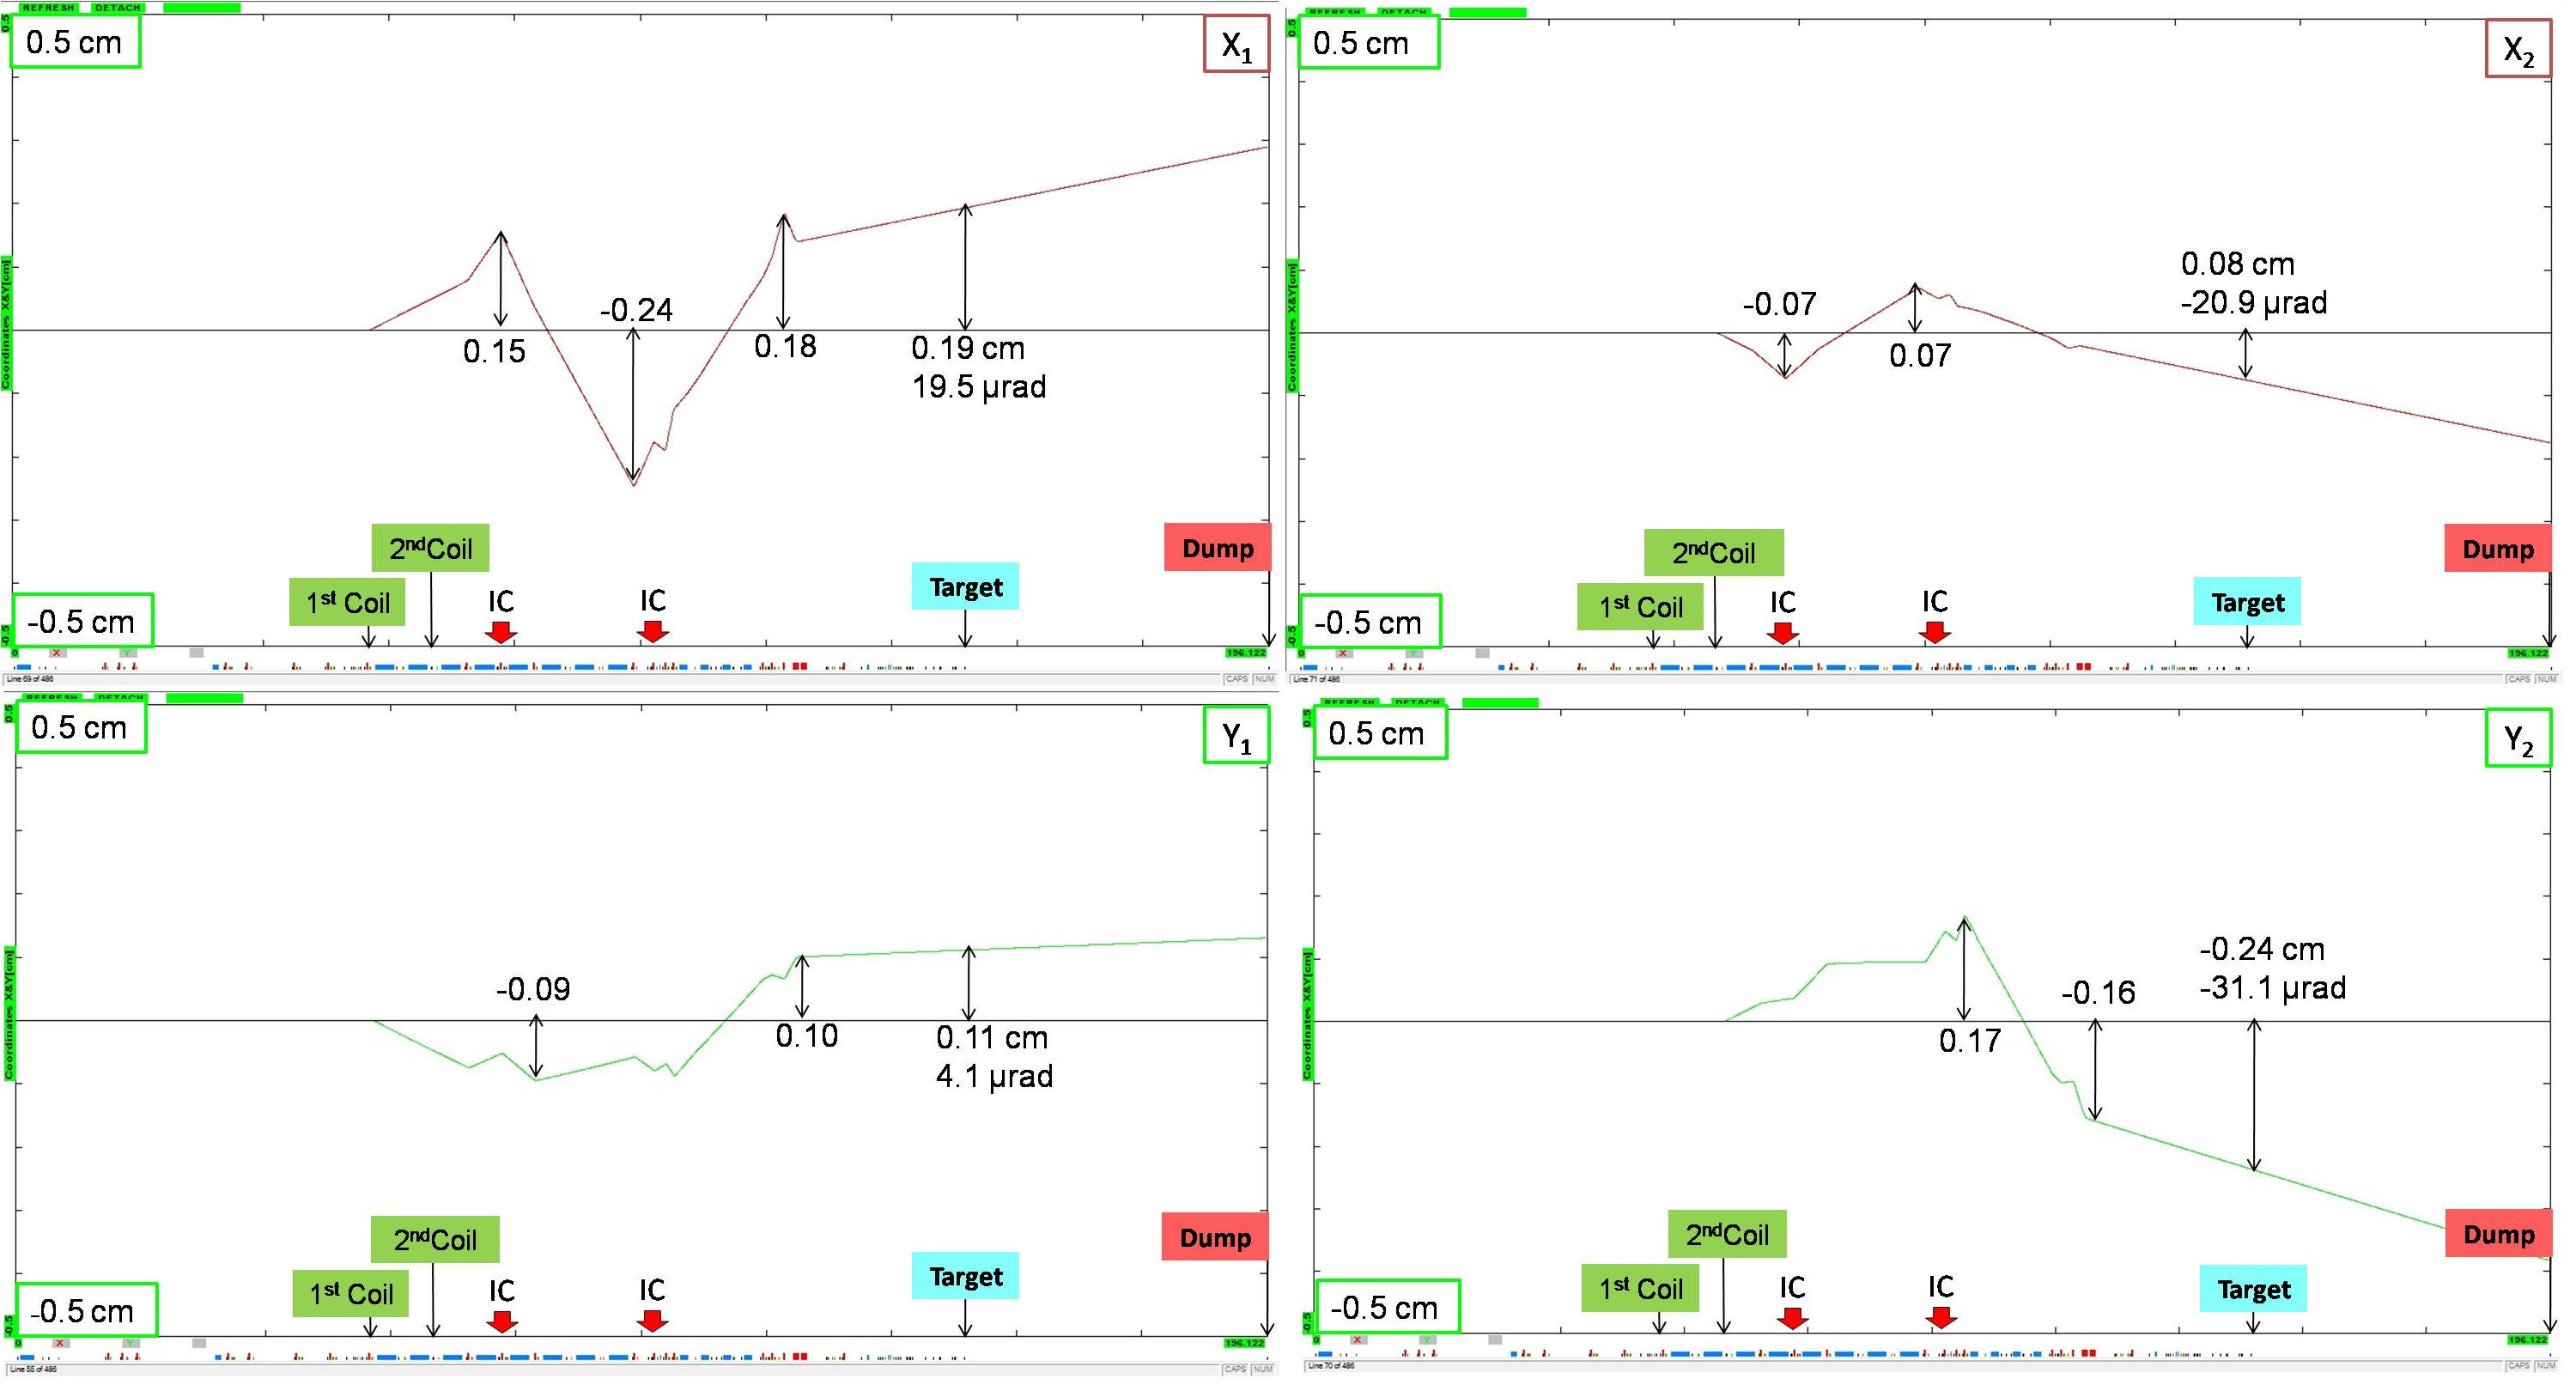
\includegraphics[width=15.0cm]{figures/BModMachineProtectionAllSingle}
	\end{center}
	\caption
	[Orbit excursions with only one coil energized.]
	{Orbit excursions with only one coil energized. Beam moves from left to right. Large excursions were observed for $X_{1}$ and $Y_{2}$ coils. The maximum current used for all the coils was $I_\textrm{max}$ = 0.6~A. A hard coded restriction of $I_\textrm{max}$ = 0.3~A in the software was set for the safety of the accelerator based on this analysis.
	}
	\label{fig:BModMachineProtectionAllSingle}
\end{figure}
\end{singlespace}



\begin{singlespace}
\begin{figure}[!h]
	\begin{center}
	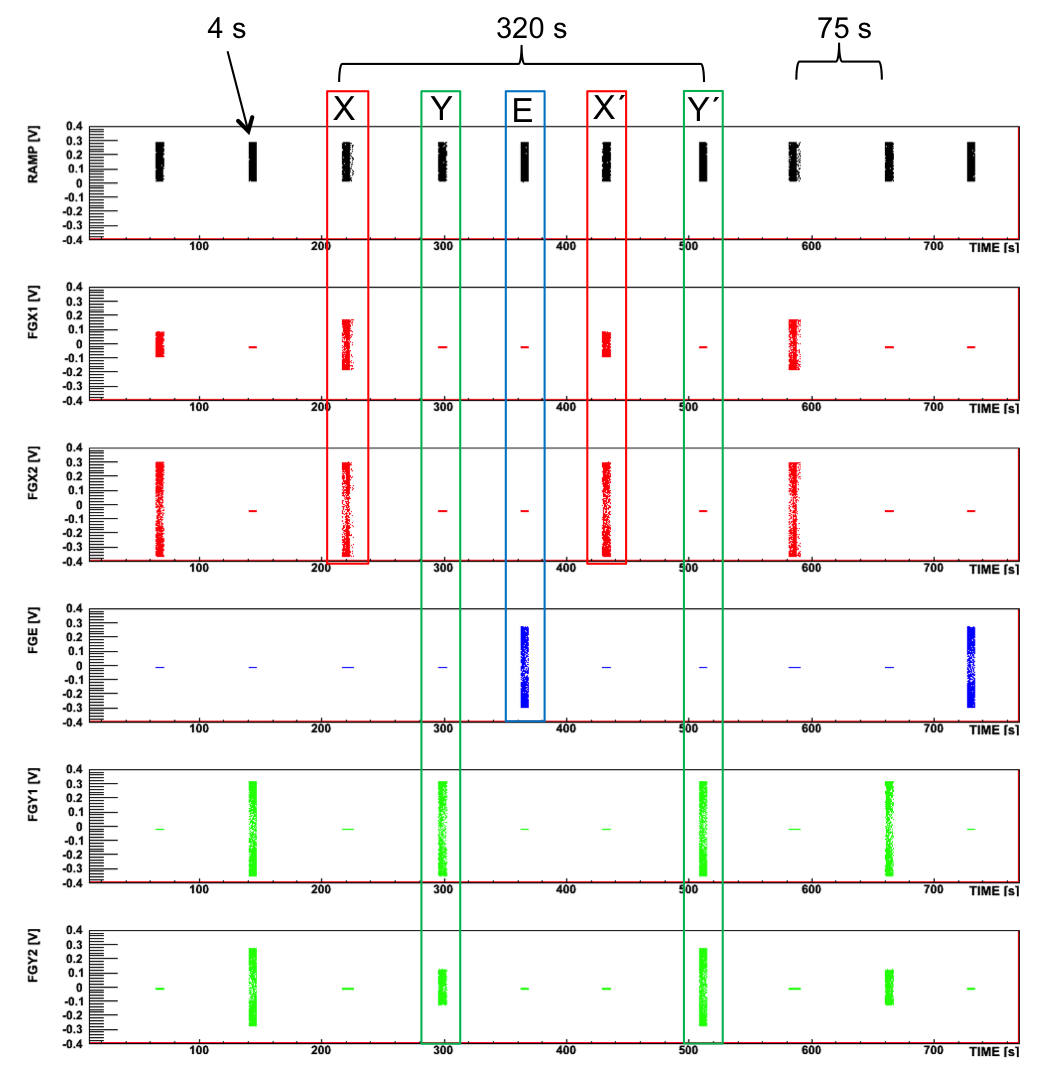
\includegraphics[width=15.0cm]{figures/BModCycle}
	\end{center}
	\caption
	[Beam modulation cycle during a typical production run.]
	{Beam modulation cycle during a typical production run. 1st panel shows ramp wave to calibrate sinusoidal signals vs time. 2nd and 3rd panels show sinusoidal drive signals for horizontal position ($X$) and angle ($X^{\prime}$) modulation vs time. 4th panel shows sinusoidal drive signals for energy ($E$) modulation vs time. 5th and 6th panels show sinusoidal drive signals for vertical position ($Y$) and angle ($Y^{\prime}$) modulation vs time. The cycle for each parameter is $\sim$4~s. One macro cycle consists of the $X$, $X^{\prime}$, $E$, $Y$, $Y^{\prime}$ cycles and ran for 320~s.}
	\label{fig:BModCycle}
\end{figure}
\end{singlespace}

%%%%%%%%%%%%%%%%%%%%%%%%%%%%%%%%%%%%%%%%%%%%%%%%%%%%%%%%%%%%%
\section{Beam Modulation Cycle}
\label{Beam Modulation Cycle}
A typical beam modulation cycle vs time during production run is shown in Figure~\ref{fig:BModCycle}. A micro cycle ran for 510~cycles with a nominal frequency of 125~Hz for each beam parameter. So the cycle for each parameter was $\sim$4~s. One macro cycle consisted of the $X$, $X^{\prime}$, $E$, $Y$, $Y^{\prime}$ cycles and ran for 320~s. Each macro cycle was then continuously repeated. The configuration time between each micro cycle was $\sim$75~s. Modulation ran with a duty factor of $\sim$6\%.
A zoomed version of the ramp and sinusoidal drive signal from the Figure~\ref{fig:BModCycle} is shown in Figure~\ref{fig:BModSignalZoomed}.

%1st panel shows ramp wave to calibrate sinusoidal signals vs time. 2nd and 3rd panel show sinusoidal drive signals for horizontal position (X) and angle (X$^{\prime}$) modulation vs time. 4th panel shows sinusoidal drive signals for energy (E) modulation vs time. 5th and 6th panel show sinusoidal drive signal for vertical position (Y) and angle (Y$^{\prime}$) modulation vs time. The cycle for each parameter was $\sim$4 s. One macro cycle consists of the X, X$^{\prime}$, E, Y, Y$^{\prime}$ cycles and ran for 320 s. Each macro cycle was then continuously repeated. 

\begin{singlespace}
\begin{figure}[!h]
	\begin{center}
	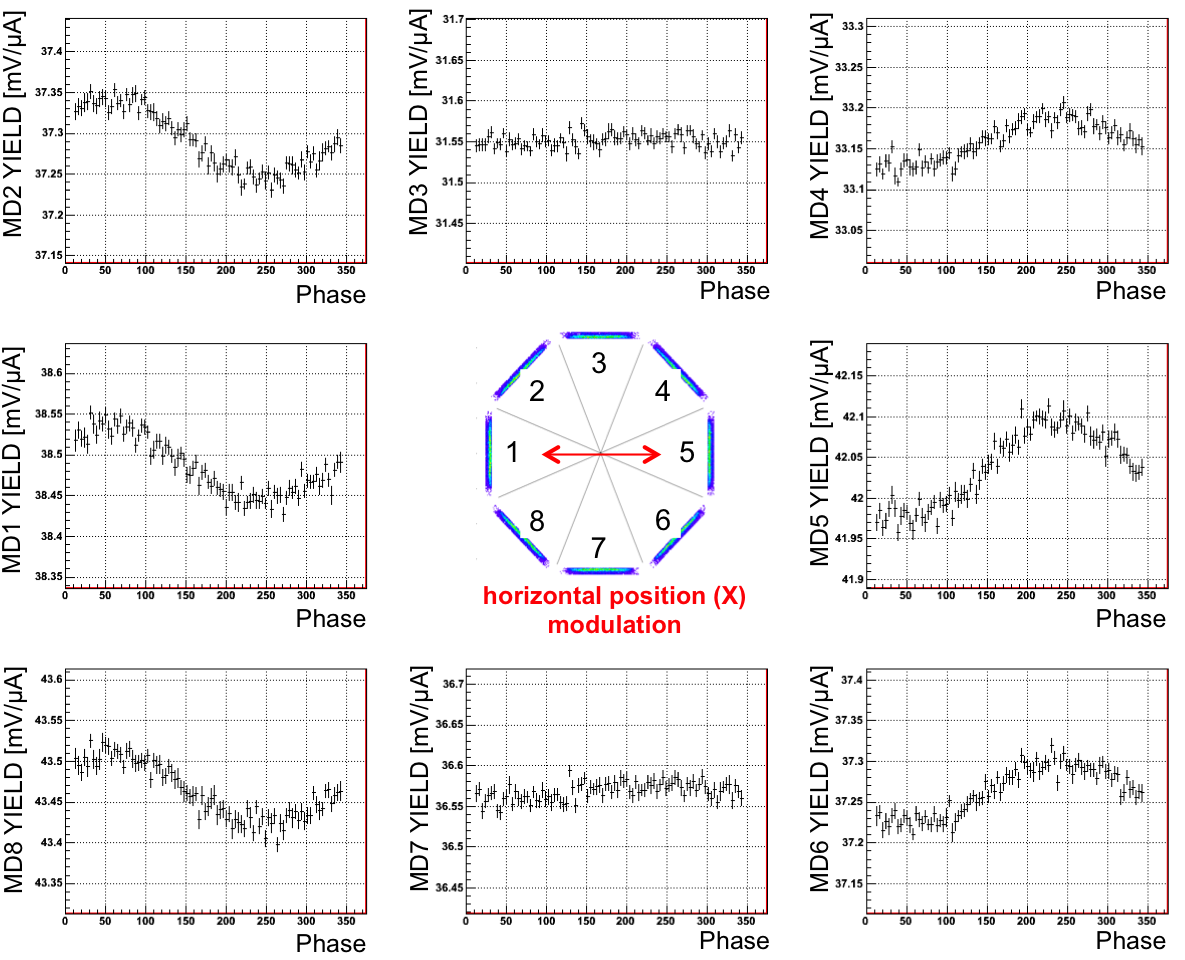
\includegraphics[width=15.0cm]{figures/BModDetectorResponse}
	\end{center}
	\caption
	[Main detector response to $X$ position modulation.]
	{Main detector response to $X$ position modulation. Main detector yields vs modulation phase (ramp wave) plotted for each detector. }
	\label{fig:BModDetectorResponse}
\end{figure}
\end{singlespace}

%%%%%%%%%%%%%%%%%%%%%%%%%%%%%%%%%%%%%%%%%%%%%%%%%%%%%%%%%%%%%
\section{Response to Modulation Signal and Applications}
\label{Response to Modulation Signal and Applications}
Main detector response to horizontal position ($X$) modulation is shown in Figure~\ref{fig:BModDetectorResponse}. The detector coordinate is shown in the center of the figure. Detectors 1 and 5 show the maximum response for the $X$ modulation and are anti correlated to each other. Negligible response has been seen in octants 3 and 7. Detector responses correlated with modulation were used to extract sensitivities for the main detector and are discussed in the next chapter. 

A typical BPM response to nominal modulation drive signal is a sinusoidal of amplitude $\sim$200~$\mu$m, as shown in Figure~\ref{fig:BModBPMResponse}. Compared with natural beam jitter, this is an order of magnitude larger and has fewer correlations among the parameters, providing an independent way of measuring sensitivities. Figure~\ref{fig:BModBPMResponse} shows a pair of drive signals for $X$ modulation in top two panels, whereas the target BPM $X$ and $Y$ responses are shown in the bottom two panels. As expected, the BPM $X$ shows a significant sinusoidal response to the horizontal drive signal but no response in $Y$. Besides measuring sensitivities, the BPM response to the modulation signal helped to track any optics change in the Hall-C beamline. The following chapter will discuss the application and products of the beam modulation system.

\begin{singlespace}
\begin{figure}[!h]
	\begin{center}
	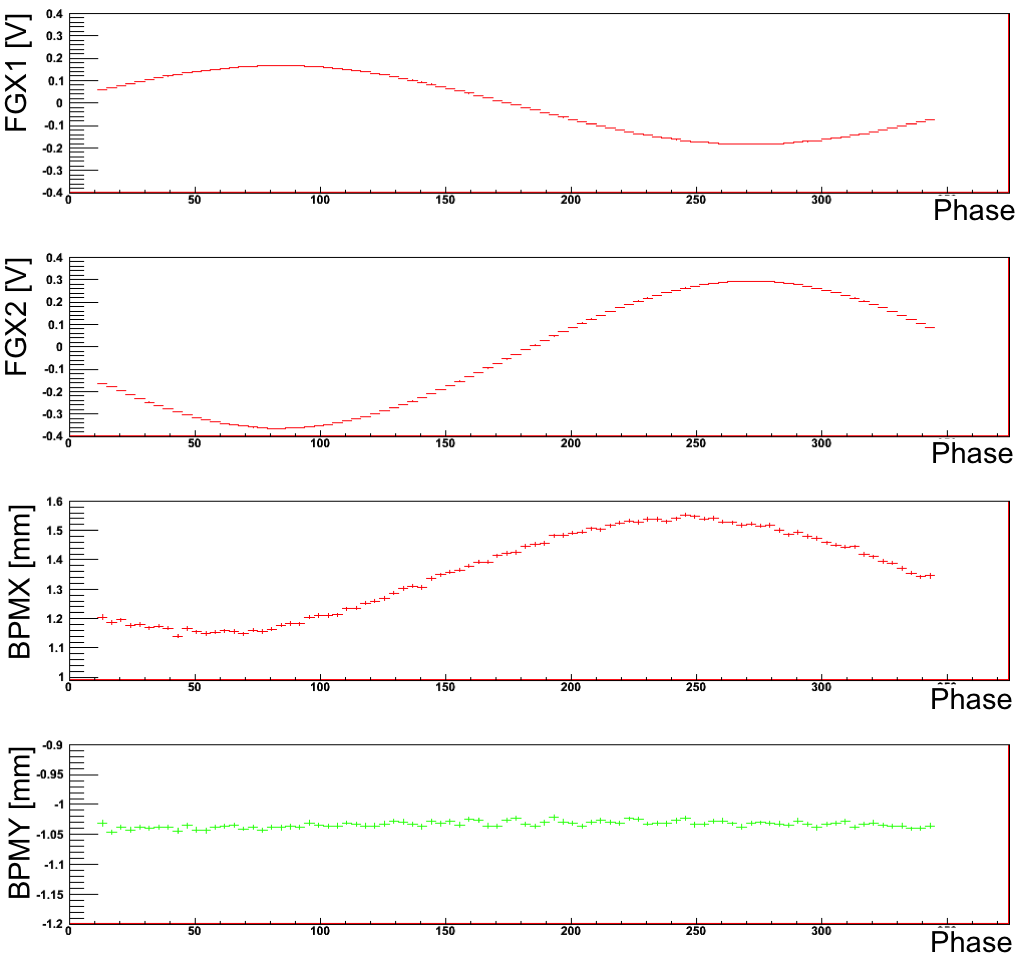
\includegraphics[width=10.0cm]{figures/BModBPMResponse}
	\end{center}
	\caption
	[Target BPM response to $X$ position modulation.]
	{Target BPM response to $X$ position modulation. The signals were plotted vs modulation phase. The drive signals in coils $X_{1}$, and $X_{2}$ are shown in top two panels and the corresponding BPM response in $X$, and $Y$ are shown in bottom two panels.}
	\label{fig:BModBPMResponse}
\end{figure}
\end{singlespace}

%%%%%%%%%%%%%%%%%%%%%%%%%%%%%%%%%%%%%%%%%%%%%%%%%%%%%%%%%%%%%
\section{Extension to Other JLab Parity Violation Experiments}
\label{Extension to Other JLab Parity Violation Experiments}
The beam modulation system described in this chapter should be useful for other parity violation experiments such as the Moeller experiment at 11~GeV in Hall-A, JLab ~\cite{moller_2010}. Some basic limitations should be kept in mind. First of all, the modulation amplitude of the system described here will scale like $E_\textrm{beam}$ (GeV)/1.165, hence the amplitudes at 11~GeV will be smaller by an order of magnitude. If the amplitude becomes smaller than the random beam jitter, convergence will be greatly slowed. The air-core coils can be driven harder if the duty factor is limited or if fans are used to cool the coils, but at about 5~A (rms) they become hot enough to risk damaging the enamel coatings on the wires under continuous duty. Secondly, at the frequencies of interest, the coil is an almost purely inductive load, so the voltage needed to drive a given current is nearly proportional to frequency. If one wishes to modulate the beam faster than the 250~Hz system described here, faster, higher voltage power amplifiers than the Trim-II would be needed. Alternatively, larger field integrals could be obtained for a given current by replacing air-core coils with ferrite magnets. Finally, because the final quadrupole is closer to the target in the Hall-A beamline (1C) line~\cite{nur_halla_beamline}, it should be somewhat easier to generate a given angle kick at a given beam energy as compared to the 3C line. 

%%%%%%%%%%%%%%%%%%%%%%%%%%%%%%%%%%%%%%%%%%%%%%%%%%%%%%%%%%%%%%
%\section{Applications of Beam Modulation System}
%\label{Applications of Beam Modulation System}
%A typical BPM response is a sinusoidal of amplitude $\sim$200~$\mu$m. Compared with natural beam jitter, this is an order of magnitude larger and has fewer correlations among the parameters, providing an independent way of measuring sensitivities. Beside measuring sensitivities, the BPM response to the modulation signal helped to track any optics change in the Hall-C beamline. Following chapter will discuss the application and products of beam modulation system.

%%%%%%%%%%%%%%%%%%%%%%%%%%%%%%%%%%%%%%%%%%%%%%%%%%%%%%%%%%%%%
\section{Summary}
\label{Summary}
The beam modulation system presented here was designed for sinusoidal modulation up to 250~Hz which was robust and well-suited for experiments measuring small parity violating asymmetries like the Q-weak experiment. At the cost of 1\% of beam time for one parameter, the system was able to measure all sensitivities to 10\% accuracy each day. The pairs of coils were tuned to deliver relatively pure positions or angle modulations, making it much less likely that singular matrices are encountered when solving for the sensitivities. The ratio of coil currents was adjusted to incorporate any optics change in the beamline compare to move the coils physically, which made the system independent of the design optic. For 1.165~GeV electron beam, using 125~Hz sinusoidal drive signal, the Trim power amplifier was able to provide the desired beam modulation amplitudes with existing air-core HF (MAT) coils. The modulation system worked quite well for the span of two years during the Q-weak experiment and collected data noninvasively with production running. However, to providing similar amplitudes for the Moller PV experiment at 12~GeV in Hall-A may require an upgrade of the amplifier or magnets. 

